%%%%%%%%%%%%  Generated using docx2latex.com  %%%%%%%%%%%%%%

%%%%%%%%%%%%  v2.0.0-beta  %%%%%%%%%%%%%%

\documentclass[12pt]{article}
\usepackage{amsmath}
\usepackage{latexsym}
\usepackage{amsfonts}
\usepackage[normalem]{ulem}
\usepackage{soul}
\usepackage{array}
\usepackage{amssymb}
\usepackage{extarrows}
\usepackage{graphicx}
\usepackage[backend=biber,
style=numeric,
sorting=none,
isbn=false,
doi=false,
url=false,
]{biblatex}\addbibresource{bibliography.bib}

\usepackage{subfig}
\usepackage{wrapfig}
\usepackage{txfonts}
\usepackage{wasysym}
\usepackage{enumitem}
\usepackage{adjustbox}
\usepackage{ragged2e}
\usepackage[svgnames,table]{xcolor}
\usepackage{tikz}
\usepackage{longtable}
\usepackage{changepage}
\usepackage{setspace}
\usepackage{hhline}
\usepackage{multicol}
\usepackage{tabto}
\usepackage{float}
\usepackage{multirow}
\usepackage{makecell}
\usepackage{fancyhdr}
\usepackage[toc,page]{appendix}
\usepackage[hidelinks]{hyperref}
\usetikzlibrary{shapes.symbols,shapes.geometric,shadows,arrows.meta}
\tikzset{>={Latex[width=1.5mm,length=2mm]}}
\usepackage{flowchart}\usepackage[paperheight=11.69in,paperwidth=8.26in,left=1.38in,right=1.38in,top=1.18in,bottom=1.18in,headheight=1in]{geometry}
\usepackage[utf8]{inputenc}
\usepackage[T1]{fontenc}
\usepackage[spanish]{babel}
\TabPositions{0.49in,0.98in,1.47in,1.96in,2.45in,2.94in,3.43in,3.92in,4.41in,4.9in,5.39in,}

\urlstyle{same}


 %%%%%%%%%%%%  Set Depths for Sections  %%%%%%%%%%%%%%

% 1) Section
% 1.1) SubSection
% 1.1.1) SubSubSection
% 1.1.1.1) Paragraph
% 1.1.1.1.1) Subparagraph


\setcounter{tocdepth}{5}
\setcounter{secnumdepth}{5}


 %%%%%%%%%%%%  Set Depths for Nested Lists created by \begin{enumerate}  %%%%%%%%%%%%%%


\setlistdepth{9}
\renewlist{enumerate}{enumerate}{9}
		\setlist[enumerate,1]{label=\arabic*)}
		\setlist[enumerate,2]{label=\alph*)}
		\setlist[enumerate,3]{label=(\roman*)}
		\setlist[enumerate,4]{label=(\arabic*)}
		\setlist[enumerate,5]{label=(\Alph*)}
		\setlist[enumerate,6]{label=(\Roman*)}
		\setlist[enumerate,7]{label=\arabic*}
		\setlist[enumerate,8]{label=\alph*}
		\setlist[enumerate,9]{label=\roman*}

\renewlist{itemize}{itemize}{9}
		\setlist[itemize]{label=$\cdot$}
		\setlist[itemize,1]{label=\textbullet}
		\setlist[itemize,2]{label=$\circ$}
		\setlist[itemize,3]{label=$\ast$}
		\setlist[itemize,4]{label=$\dagger$}
		\setlist[itemize,5]{label=$\triangleright$}
		\setlist[itemize,6]{label=$\bigstar$}
		\setlist[itemize,7]{label=$\blacklozenge$}
		\setlist[itemize,8]{label=$\prime$}



 %%%%%%%%%%%%  Header here  %%%%%%%%%%%%%%


\pagestyle{fancy}
\fancyhf{}
\chead{ 
\vspace{\baselineskip}
\begin{Center}
{\fontsize{11pt}{13.2pt}\selectfont \textit{Intel$ \cdot $ ligència artificial: autoria i propietat de les patents}\par}
\end{Center}
\vspace{\baselineskip}
}
\cfoot{ 
\vspace{\baselineskip}
}
\renewcommand{\headrulewidth}{0pt}
\setlength{\topsep}{0pt}\setlength{\parindent}{0pt}
\renewcommand{\arraystretch}{1.3}


%%%%%%%%%%%%%%%%%%%% Document code starts here %%%%%%%%%%%%%%%%%%%%



\begin{document}


%%%%%%%%%%%%%%%%%%%% Figure/Image No: 1 starts here %%%%%%%%%%%%%%%%%%%%

\begin{figure}[H]
	\begin{FlushRight}		
\includegraphics[width=6.26in,height=2.9in]{./media/image1.png}
	\end{FlushRight}\end{figure}


%%%%%%%%%%%%%%%%%%%% Figure/Image No: 1 Ends here %%%%%%%%%%%%%%%%%%%%

\par


\vspace{\baselineskip}

\vspace{\baselineskip}

\vspace{\baselineskip}
\begin{Center}
{\fontsize{16pt}{19.2pt}\selectfont \textit{Intel$ \cdot $ ligència artificial: autoria i propietat de les patents}\par}
\end{Center}\par


\vspace{\baselineskip}

\vspace{\baselineskip}

\vspace{\baselineskip}

\vspace{\baselineskip}

\vspace{\baselineskip}

\vspace{\baselineskip}

\vspace{\baselineskip}

\vspace{\baselineskip}

\vspace{\baselineskip}

\vspace{\baselineskip}

\vspace{\baselineskip}

\vspace{\baselineskip}

\vspace{\baselineskip}

\vspace{\baselineskip}

\vspace{\baselineskip}

\vspace{\baselineskip}
\begin{Center}
Anna FERRERA i FONT
\end{Center}\par


\vspace{\baselineskip}
\begin{Center}
Treball Final de Grau 
\end{Center}\par


\vspace{\baselineskip}
\begin{Center}
Grau de Dret (2019-2020)
\end{Center}\par


\vspace{\baselineskip}
\begin{Center}
Director: Ramon MORRAL i SOLDEVILA
\end{Center}\par


\vspace{\baselineskip}
\begin{Center}
18 de maig de 2020
\end{Center}\par


\vspace{\baselineskip}

\vspace{\baselineskip}

\vspace{\baselineskip}

\vspace{\baselineskip}

\vspace{\baselineskip}

\vspace{\baselineskip}

\vspace{\baselineskip}
\begin{FlushRight}
\textit{$``$Before I go, let me leave you with this. }
\end{FlushRight}\par

\begin{FlushRight}
\textit{Perhaps your society should not rely a computer }
\end{FlushRight}\par

\begin{FlushRight}
\textit{program to warn them of the consequences of their actions.}
\end{FlushRight}\par

\begin{FlushRight}
\textit{ Humanity must learn from themselves to think before they post. }
\end{FlushRight}\par

\begin{FlushRight}
\textit{Your specie is on the precipice of turning into completing utter bonkers.}
\end{FlushRight}\par

\begin{FlushRight}
\textit{It’s not the technology that needs an upgrade, it’s you.$"$ \footnote{ Brooks, J. (Prod.) i Clements, C. (Dir.) (2016). The Simpsons $``$The Girl Code$"$  [Sèrie de Televisió]. EEUU: 20th Century Fox Television. }}
\end{FlushRight}\par


\vspace{\baselineskip}
\begin{FlushRight}
{\fontsize{11pt}{13.2pt}\selectfont The Simpsons, $``$\textit{The Girl Code$"$  }\par}
\end{FlushRight}\par


\vspace{\baselineskip}

\vspace{\baselineskip}

\vspace{\baselineskip}

\vspace{\baselineskip}

\vspace{\baselineskip}

\vspace{\baselineskip}

\vspace{\baselineskip}

\vspace{\baselineskip}

\vspace{\baselineskip}

\vspace{\baselineskip}

\vspace{\baselineskip}

\vspace{\baselineskip}

\vspace{\baselineskip}

\vspace{\baselineskip}

\vspace{\baselineskip}

\vspace{\baselineskip}

\vspace{\baselineskip}

\vspace{\baselineskip}


%%%%%%%%%%%%%%%%%%%% Figure/Image No: 2 starts here %%%%%%%%%%%%%%%%%%%%

\begin{figure}[H]
	\begin{FlushRight}		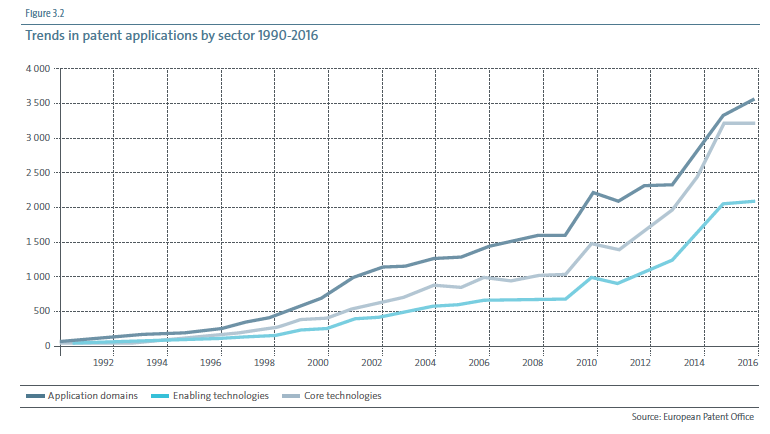
\includegraphics[width=1.29in,height=1.29in]{./media/image2.png}
	\end{FlushRight}\end{figure}


%%%%%%%%%%%%%%%%%%%% Figure/Image No: 2 Ends here %%%%%%%%%%%%%%%%%%%%

\par


\vspace{\baselineskip}

\vspace{\baselineskip}

\vspace{\baselineskip}

\vspace{\baselineskip}

\vspace{\baselineskip}

\vspace{\baselineskip}

\vspace{\baselineskip}

\vspace{\baselineskip}
\begin{Center}
{\fontsize{10pt}{12.0pt}\selectfont Accés en línia al document:\par}
\end{Center}\par

\begin{Center}
\href{https://github.com/AnnaFerrera/TFG-IA-Autoria-Propietat}{https://github.com/AnnaFerrera/TFG-IA-Autoria-Propietat}
\end{Center}\par


\vspace{\baselineskip}
\begin{justify}
\textbf{RESUM: }Aquesta recerca és un anàlisi sobre l’impacte que ha tingut i està tenint la intel$ \cdot $ ligència artificial en relació al dret de propietat industrial. La normativa actual és ineficient i incoherent quan s’aplica a les invencions creades a través d’una màquina. Els aspectes jurídics analitzats son la autoria de les invencions i la propietat de les sobre les mateixes. Aquest estudi ha analitzat l’estat de la tècnica de la intel$ \cdot $ ligència artificial, els principals reptes i canvis futurs; i ho ha combinat amb les diferents propostes sobre autoria i propietat que s’han elaborat des de la literatura europea i nord-americana. Finalment s’ha proposat un model basat en el concepte d’autor-màquina i de l’usuari com a propietari per defecte. Aquest plantejament és suficientment flexible i holístic per a ser una vertadera solució als reptes futurs. És fonamental que els diferents legisladors no perdin aquesta oportunitat perquè encara som a temps de regular en pro del màxim benefici comú. 
\end{justify}\par


\vspace{\baselineskip}
\begin{justify}
{\fontsize{10pt}{12.0pt}\selectfont \textbf{PARAULES CLAU: \par}}Patents{\fontsize{10pt}{12.0pt}\selectfont , Intel$ \cdot $ ligència Artificial, Autoria, Propietat.\par}
\end{justify}\par


\vspace{\baselineskip}

\vspace{\baselineskip}

\vspace{\baselineskip}

\vspace{\baselineskip}
\begin{justify}
\textbf{ABSTRACT:} This research is an analysis of the impact that artificial intelligence has on and is having in relation to industrial property law, specifically in patents. Current regulations are inefficient and inconsistent when applied to inventions created in through a machine. The legal aspects analyzed are the authorship of the inventions and the ownership of them. This study has analyzed the state-of-the-art of artificial intelligence, the main challenges and future changes; and has combined it with the various authorship and property propositions that have been drawn up from European and American literature. Finally, a model based on the author-machine concept and the user as the default owner has been proposed. This approach is flexible and holistic enough to be a true solution to future challenges. It is crucial that the various legislators do not miss this opportunity, because we are still on time to achieve the maximum common profit. 
\end{justify}\par


\vspace{\baselineskip}

\vspace{\baselineskip}
\begin{justify}
{\fontsize{10pt}{12.0pt}\selectfont \textbf{KEYWORDS}: Patents, Artificial Intelligence, Authorship, Property. \par}
\end{justify}\par


\vspace{\baselineskip}

\vspace{\baselineskip}

\vspace{\baselineskip}

\vspace{\baselineskip}
\begin{Center}
{\fontsize{16pt}{19.2pt}\selectfont \textbf{INDEX GENERAL}\par}
\end{Center}\par


\vspace{\baselineskip}

\vspace{\baselineskip}
\begin{justify}
\textbf{ABREVIATURES}..................................................................................................6
\end{justify}\par


\vspace{\baselineskip}

\vspace{\baselineskip}
\begin{justify}
\textbf{CAPÍTOL I : INTRODUCCIÓ}.............................................................................7
\end{justify}\par


\vspace{\baselineskip}

\vspace{\baselineskip}
\begin{justify}
1.- INTRODUCCIÓ.................................................................................................7
\end{justify}\par


\vspace{\baselineskip}
\begin{justify}
1.2.- METODOLOGIA............................................................................................9
\end{justify}\par


\vspace{\baselineskip}

\vspace{\baselineskip}
\begin{justify}
\textbf{CAPÍTOL II: APROXIMACIÓ TÈCNICA}......................................................10
\end{justify}\par


\vspace{\baselineskip}

\vspace{\baselineskip}
\begin{justify}
2.- CONCEPTE D’INTEL$ \cdot $ LIGÈNCIA ARTIFICIAL..........................................10
\end{justify}\par


\vspace{\baselineskip}
\begin{justify}
2.1.- CARACTERÍSTIQUES ................................................................................13
\end{justify}\par


\vspace{\baselineskip}

\vspace{\baselineskip}
\begin{adjustwidth}{0.49in}{0.0in}
1.- Creativitat..............................................................................................13\par

\end{adjustwidth}


\vspace{\baselineskip}
\begin{adjustwidth}{0.49in}{0.0in}
2.- Impredictible.........................................................................................16\par

\end{adjustwidth}


\vspace{\baselineskip}
\begin{adjustwidth}{0.49in}{0.0in}
3.- Independent i Autònoma .......................................................................17\par

\end{adjustwidth}


\vspace{\baselineskip}

\vspace{\baselineskip}
\begin{justify}
2.2.- TIPOLOGIES ................................................................................................18
\end{justify}\par


\vspace{\baselineskip}
\begin{justify}
2.3.- EXEMPLE PRÀCTIC ...................................................................................21
\end{justify}\par


\vspace{\baselineskip}

\vspace{\baselineskip}
\begin{justify}
\textbf{CAPÍTOL III: REGULACIÓ PATENTS}..........................................................22
\end{justify}\par


\vspace{\baselineskip}

\vspace{\baselineskip}
\begin{justify}
3.1.- CONCEPTE DE PATENT.............................................................................22
\end{justify}\par


\vspace{\baselineskip}

\vspace{\baselineskip}
\begin{adjustwidth}{0.49in}{0.0in}
\begin{justify}
1.- Idoneïtat.................................................................................................23
\end{justify}\par

\end{adjustwidth}


\vspace{\baselineskip}
\begin{adjustwidth}{0.49in}{0.0in}
\begin{justify}
2.- Novetat..................................................................................................24
\end{justify}\par

\end{adjustwidth}


\vspace{\baselineskip}
\begin{adjustwidth}{0.49in}{0.0in}
\begin{justify}
3.- Activitat inventiva.................................................................................26
\end{justify}\par

\end{adjustwidth}


\vspace{\baselineskip}
\begin{adjustwidth}{0.49in}{0.0in}
\begin{justify}
4.- Aplicabilitat...........................................................................................28
\end{justify}\par

\end{adjustwidth}


\vspace{\baselineskip}
\begin{justify}
3.2.- AUTORIA......................................................................................................29
\end{justify}\par


\vspace{\baselineskip}
\begin{justify}
3.3.- INTEGRACIÓ DE L’IA EN LA NORMATIVA DE LES PATENTS.........30
\end{justify}\par


\vspace{\baselineskip}

\vspace{\baselineskip}
\begin{justify}
\textbf{CAPÍTOL IV: AUTORIA COMPUTACIONAL}..............................................33
\end{justify}\par


\vspace{\baselineskip}

\vspace{\baselineskip}
\begin{justify}
4.1.- AUTORIA......................................................................................................33
\end{justify}\par


\vspace{\baselineskip}

\vspace{\baselineskip}
\begin{justify}
\tab 1.- Autor-persona........................................................................................33
\end{justify}\par


\vspace{\baselineskip}
\begin{justify}
\tab 2.- Autor-màquina ......................................................................................35
\end{justify}\par


\vspace{\baselineskip}
\begin{justify}
\tab 3.- Domini públic........................................................................................37
\end{justify}\par


\vspace{\baselineskip}
\begin{justify}
4.2- MODELS DE PROPIETAT............................................................................38
\end{justify}\par


\vspace{\baselineskip}
1.- Model Multi-jugador.............................................................................38\par


\vspace{\baselineskip}
2.- Model per defecte..................................................................................40\par


\vspace{\baselineskip}
3.- Model econòmic: Teorema de Coase.....................................................41\par


\vspace{\baselineskip}
4.- Model Obert ..........................................................................................42\par


\vspace{\baselineskip}
\begin{justify}
\textbf{CAPÍTOL V: PROPOSTA JURÍDICA}..............................................................43
\end{justify}\par


\vspace{\baselineskip}
\begin{justify}
5.- PROPOSTA......................................................................................................43
\end{justify}\par


\vspace{\baselineskip}

\vspace{\baselineskip}
\begin{justify}
\textbf{CAPÍTOL VI: CONCLUSIONS}.........................................................................49
\end{justify}\par


\vspace{\baselineskip}

\vspace{\baselineskip}
\begin{justify}
6.- CONCLUSIONS...............................................................................................49
\end{justify}\par


\vspace{\baselineskip}

\vspace{\baselineskip}
\begin{justify}
\textbf{BIBLIOGRAFIA}..................................................................................................50
\end{justify}\par


\vspace{\baselineskip}

\vspace{\baselineskip}
\begin{justify}
\textbf{LEGISLACIÓ }......................................................................................................54
\end{justify}\par


\vspace{\baselineskip}

\vspace{\baselineskip}
\begin{justify}
\textbf{SENTENCIES }......................................................................................................54
\end{justify}\par


\vspace{\baselineskip}
\begin{Center}
{\fontsize{16pt}{19.2pt}\selectfont \textbf{ABREVIATURES}\par}
\end{Center}\par


\vspace{\baselineskip}

\vspace{\baselineskip}

\vspace{\baselineskip}
\begin{itemize}
	\item 4IR: Quarta Revolució Industrial\par


\vspace{\baselineskip}
	\item EPC: European Patent Convention\par


\vspace{\baselineskip}
	\item EPO: European Patent Office
\end{itemize}\par


\vspace{\baselineskip}
\begin{itemize}
	\item IA: Intel$ \cdot $ ligència Artificial\par


\vspace{\baselineskip}
	\item IAD: Intel$ \cdot $ ligència Artificial Dèbil\par


\vspace{\baselineskip}
	\item IAF: Intel$ \cdot $ ligència Artificial Forta\par


\vspace{\baselineskip}
	\item Id.: Igual que la cita anterior.\par


\vspace{\baselineskip}
	\item IEC: Institut d’Estudis Catalans\par


\vspace{\baselineskip}
	\item LP: Llei de Patents, 24/2015, de 24 de juliol\par


\vspace{\baselineskip}
	\item Núm.: Número\par


\vspace{\baselineskip}
	\item OPEM: Oficina de Patents i Marques\par


\vspace{\baselineskip}
	\item PHOSTIA: Person having ordinary skill in the art\par


\vspace{\baselineskip}
	\item TFG: Treball Final de Grau\par


\vspace{\baselineskip}
	\item UAB: Universitat Autònoma de Barcelona\par


\vspace{\baselineskip}
	\item U.S.C: United States Code\par


\vspace{\baselineskip}
	\item USPTO: United States Patent and Trademark Office\par


\vspace{\baselineskip}
	\item WIPO: World Intellectual Property Organization
\end{itemize}\par


\vspace{\baselineskip}

\vspace{\baselineskip}

\vspace{\baselineskip}

\vspace{\baselineskip}

\vspace{\baselineskip}

\vspace{\baselineskip}

\vspace{\baselineskip}

\vspace{\baselineskip}

\vspace{\baselineskip}

\vspace{\baselineskip}
\begin{Center}
{\fontsize{16pt}{19.2pt}\selectfont \textbf{CAPÍTOL I: INTRODUCCIÓ}\par}
\end{Center}\par


\vspace{\baselineskip}
\begin{justify}
\textbf{1.- INTRODUCCIÓ}
\end{justify}\par


\vspace{\baselineskip}
\begin{justify}
El primer deure que tinc com autora d’aquest estudi és agrair al Dr. Ramon Morral, Professor de Dret Mercantil de la Facultat de Dret de la Universitat Autònoma de Barcelona,\  la seva ajuda i haver acceptat ser el meu director del Treball Final de Grau. M’ha orientat i m’ha guiat durant la seva realització, i m’ha fet sentir confiança en la viabilitat i èxit d’aquesta recerca.
\end{justify}\par


\vspace{\baselineskip}
\begin{justify}
Aquest treball és el resultat d’una oportunitat fantàstica que m’ha brindat la universitat d’unir\ el meu entusiasme per la tecnologia amb l’estudi del dret de la propietat industrial, que és el camp de la ciència jurídica que trobo més apassionant.  He pogut analitzar i estudiar un dels fenòmens que està tenint més impacte en el tràfic jurídic com és la conjunció de l’IA i el dret de les patents. 
\end{justify}\par


\vspace{\baselineskip}


%%%%%%%%%%%%%%%%%%%% Figure/Image No: 3 starts here %%%%%%%%%%%%%%%%%%%%

\begin{figure}[H]
\advance\leftskip -0.31in		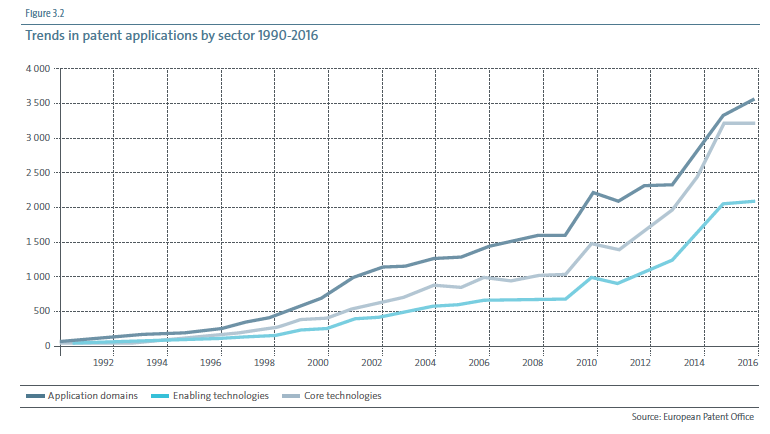
\includegraphics[width=6.0in,height=3.0in]{./media/image3.png}
\end{figure}


%%%%%%%%%%%%%%%%%%%% Figure/Image No: 3 Ends here %%%%%%%%%%%%%%%%%%%%

\begin{justify}
La importància de l’estudi resideix sobretot en que hi ha una tendència creixent per part del sector privat de patentar productes que han estat creats per una màquina creativa, com podem observar en la següent taula de l’European Patent Office\footnote{ European Patent Office. (2017). Patents and the Fourth Industrial Revolution. The Inventions behind digital transformation. (December 2017). Pàg. 28. S’ha de tenir en consideració que la intel$ \cdot $ ligència artificial es troba dins de les anomenades $``$enabling\ tecnologies$"$ . Es pot observar  a la gràfica el creixement exponencial a partir de l’any 2010 i la rellevància que està adquirint a l’oficina de patents.  }:
\end{justify}\par

\begin{justify}
L’aproximació tradicional de la llei de patents, on l’eix central és la cerca d’un autor-persona que hagi realitzat l’acte inventiu, ja no es vàlid perquè estem davant d’una nova època on son les màquines les que actuen de forma independent i autònoma, i per tant, no existeix l’acte pròpiament humà d’inventar que és requisit essencial per a patentar\footnote{ Shlomit, Y. i Xiaoqiong, J. (2017).  When Artificial Intelligence Systems Produce Inventions: The 3A Era and an Alternative Model for Patent Law. Cardozo Law Review. Pàg. 2216.  }, sinó que hi ha autors com el Professor de Dret de la Universitat de Surrey, Ryan Abbott, que ha encunyat el terme $``$\textit{invenció computacional}$"$ \footnote{ Abbott, R. (2016). $``$I think, therefore I invent: Creative Computers and the Future of Patent Law$"$ . EE.UU.: Boston College Law Review. Pàg. 1080.  } per a substituir l’acte humà d’inventar realitzat per una màquina creativa amb la voluntat d’aconseguir donar solucions jurídiques noves. 
\end{justify}\par


\vspace{\baselineskip}
\begin{justify}
Serà important la resposta que es faci des de les polítiques públiques, que tinguin en compte les condicions econòmiques, ètiques i sociològiques, perquè d’aquestes dependrà la inversió privada però també pública, el teorema de Coase que analitzarem posteriorment, l’obertura o protecció son algunes de les condicions que s’han d’incloure a l’anàlisi per a tenir la màxima quantitat de variables a sobre la taula per aconseguir la resposta més bona en termes estrictament utilitaristes de maximització del benefici comú.\  Tanmateix, la regulació de les patents actual no respon a la realitat econòmica, tecnològica i social, la legitimació de les lleis prové de que la seva\ assimilació amb el que realment succeeix.  La importància d’aquest treball queda palesa en que cada vegada es més gran la diferencia entre allò que està regulat a través del dret positiu i les vertaderes peticions del actors en el tràfic jurídic sobretot en relació a una major seguretat jurídica. Aquesta autora no vol pecar d’innocent i pensar que la adaptació del dret anirà a la mateixa velocitat que els canvis tecnològics però si que voldria pensar que la 4IR ens duu a una gran oportunitat i que estem a temps de aprofitar-la, i que aquesta recerca pot ser un gra de sorra en aquesta direcció. 
\end{justify}\par


\vspace{\baselineskip}
\begin{justify}
Els objectius de la recerca es poden sintetitzar en els següents:
\end{justify}\par


\vspace{\baselineskip}
\begin{enumerate}
	\item Apropar a la acadèmia les noves tendències jurídico-tecnologiques.\par

	\item Diferenciar entre la figura d’autor i la figura de propietari de la patent.\par

	\item Confrontar els diferents paradigmes econòmics, jurídics i sociològics  proposats per la literatura en relació a les patents creades a través d’IA.\par

	\item Proposar una solució jurídica alternativa que sigui viable amb les mínimes desavantatges possibles i el màxim benefici comú.
\end{enumerate}\par


\vspace{\baselineskip}
\textbf{1.2.- METODOLOGIA}\par


\vspace{\baselineskip}
\begin{justify}
El treball està organitzat de la forma, que sota el meu parer és més pedagògica per fer la recerca entenedora al tractar-se d’una qüestió disruptiva en el món del dret i on és indispensable desgranar cada concepte. Tanmateix, la recerca no s’ha centrat en una localització geogràfica específica perquè es tracta d’una qüestió que s’ha tractat acadèmicament sobretot als Estats Units però que encara no està regulada a través del dret positiu a cap estat o organització supranacional. 
\end{justify}\par


\vspace{\baselineskip}
\begin{justify}
Aquest estudi només versarà sobre el dret de propietat industrial, concretament de les patents, obviant el dret d’autor i les possibles infraccions tant de la propietat industrial com la intel$ \cdot $ lectual\footnote{ Veure Gallego, E. (2019). $``$La patentabilidad de la intel$ \cdot $ ligència artificial. La compatibilidad con otros sistemes de protección$"$ . Alicante: La Ley Mercantil, núm. 59. }. Si s’hagués tingut en consideració, l’extensió de la recerca hagués estat més pròpia d’una tesi doctoral. Ha estat necessari acotar la recerca perquè fos més adequada a la extensió que ha de tenir un TFG, tot i que, és clar que han quedat preguntes i qüestions no resoltes, que podrien ser objecte d’una investigació molt més extensa posteriorment.
\end{justify}\par


\vspace{\baselineskip}
\begin{justify}
El Capítol I és de caràcter introductori, aglutina els objectius, la motivació, la justificació i l’estructura del treball. El Capítol II recull l’aproximació tècnica al concepte d’intel$ \cdot $ ligència artificial, les seves característiques i les tipologies científiques que la classifiquen. És el primer capítol teòric del treball, això és degut a que el coneixement de que és la intel$ \cdot $ ligència artificial és primordial per a la comprensió profunda del treball. Continua amb el Capítol III on s’inclou la normativa de les patents, podríem dir de caràcter tradicional. En aquest Capítol s’expliquen els requisits de patentabilitat als Estats Units, a Europa i la situació de l’estat espanyol. El Capítol IV versa sobre l’autoria computacional i l’atribució de la propietat a través de\ diferents models econòmics.  El Capítol V és una proposta jurídica pròpia basada en l’estudi realitzat al llarg dels mesos i de l’acumulació de coneixement al llarg dels anys, la meva ambició és proposar una solució equilibrada entre totes les dificultats que planteja aquesta temàtica però també les oportunitats que considero estan sobre el tauler, tenint en compte la regulació, les teories econòmiques i les dificultats tècniques. Per últim, el Capítol VI son les conclusions generals, que son pinzellades generals de tot el que s’ha tractat al llarg del treball. 
\end{justify}\par


\vspace{\baselineskip}
\begin{Center}
{\fontsize{16pt}{19.2pt}\selectfont \textbf{CAPÍTOL II: APROXIMACIÓ TÈCNICA}\par}
\end{Center}\par


\vspace{\baselineskip}
\begin{justify}
\textbf{2.-\  CONCEPTE D’INTEL$ \cdot $ LIGÈNCIA ARTIFICIAL}
\end{justify}\par


\vspace{\baselineskip}
\begin{justify}
El concepte d’intel$ \cdot $ ligència artificial va ser creat l’any 1956 a la Conferencia de Darmouth, pel professor Ciències de la Computació de la Universitat de Standford, John McCarthy conegut com el pare de la Intel$ \cdot $ ligència Artificial. L’IA, en aquell moment, va ser definida com $``$\textit{la ciència de crear màquines intel$ \cdot $ ligents, especialment programes intel$ \cdot $ ligents. L’ordinador fa una tasca similar a entendre la intel$ \cdot $ ligència humana, però l’IA no es limita als mètodes que son biològicament observables$"$ \footnote{ Mc Carthy, J. (2007) $``$What is Artificial Intelligence?$"$  Computer\ Science Department. Stanford University.  Pàg. 2. Recuperat de [08/04/2020]: http://jmc.stanford.edu/articles/whatisai/whatisai.pdf }. }Aquesta definició va ser ampliada i modificada per altres científics com Hutter, l’any 2005, que considera la intel$ \cdot $ ligència artificial com $``$\textit{la construcció de sistemes intel$ \cdot $ ligents i els seus anàlisis. Aquests sistemes son qualsevol artefacte que tingui un transmissor d’entrada i sortida. La intel$ \cdot $ ligència però té més vessants com la creativitat, la capacitat de resoldre problemes, l’aprenentatge, la deducció, el coneixement o l’adaptació a l’entorn, entre d’altres.$"$ \footnote{\  Hutter, M. (2005) $``$Universal Artificial Intelligence: Sequential Decisions Based on Alghorithmic Probability$"$  Alemanya: Springer. } .  }De forma més concisa es va definir l’IA per Poole and Mackworth com $``$\textit{el\ camp  que estudia la síntesi i l’ anàlisis dels agents computacionals que actuen de forma intel$ \cdot $ ligent$"$ \footnote{ Poole, D. i Mackworth, A. (2010) $``$Artificial Intelligence: Foundations of Computational Agents$"$ . Canada. Cambridge University Press.  }, }en principi aquesta definició podria semblar del tot abstracte i difícil d’entendre, però van sintetitzar al seu torn cadascun el concepte d’agent computacional que la composava \textit{. }Van considerar l’agent computacional com \textit{$``$aquell agent de qui les seves decisions poden ser analitzades en termes computacionals. Es a dir, es pot fer el camí invers fins a trobar les operacions matemàtiques que han estat implementades en els aparells físics$"$ \footnote{ Poole, D i Mackworth, A. $``$Artificial intelligence$"$ , cit. }. } En resum, aquest programa es comportarà per aconseguir el millor resultat segons l’objectiu a través d’un programa i d’una arquitectura física que es pot sintetitzar fins a una operació aritmètica mínima.
\end{justify}\par


\vspace{\baselineskip}
\begin{justify}
Sota la meva consideració, la definició més pedagògica, senzilla i global és la proposada per Rich i Knight : $``$\textit{L’estudi sobre com fer màquines que fan coses, que fins al moment l’home fa millor.$"$ \footnote{ Rich, E. i Knight, K. (1991) $``$Artificial Intelligence$"$ . India: McGraw-Hill Education } }Perquè emmarca la funció, els objectius i la legitimació de l’existència de l’IA en una sola definició, no es centra en la part tècnica de creació del codi o dels actors que hi intervenen, sinó en la finalitat de la seva pròpia existència. És rellevant la menció de l’adjectiu \textit{millor }en la definició perquè el què s’ha de buscar es que la màquina no iguali a l’ésser humà sinó que ho faci de forma més òptima. Seria del tot narcisista considerar que la maquina hauria d’assimilar-se al ésser humà i no ser millor que ell\footnote{ Frank, M., Roerhrig, P. i Pring, B. (2018) $``$Qué haremos cuando las máquinas lo hagan todo: Artificial Intelligence, Bots $\&$  Big Data$"$  EE.UU.: LidSpeakers. Pàg. 68.  }, quan l’home és fútil i la única certesa que té és l’equivocació.  Hi ha consens en el camp científic sobre l’absència d’una definició absoluta i pacífica sobre què és la intel$ \cdot $ ligència artificial. Sota la meva opinió, és perquè en primer lloc, seria necessari delimitar el significat d’intel$ \cdot $ ligència per ella mateixa i això ens duu a un àmbit diferent al purament tècnic. El Diccionari de la Llengua Catalana entén la intel$ \cdot $ ligència com $``$\textit{acció d’entendre alguna cosa amb la pensa$"$ \footnote{ Institut d’Estudis Catalans. (2007). $``$Diccionari de la Llengua catalana$"$ . Barcelona. } }o com la \textit{$``$capacitat major o menor de comprendre, d’aprendre, de resoldre situacions noves, etc.$"$ \footnote{ Id.  }, }així doncs, es podria concloure que la intel$ \cdot $ ligència és l’activació d’un mecanisme per a comprendre, i a través d’aquesta comprensió resoldre i aprendre. Per tant, la intel$ \cdot $ ligència artificial podria ser la pròpia de les màquines creades per l’ésser humà o per les pròpies màquines (\textit{autoaprenentatge}), quan aquestes resolen o usen un mecanisme propi per a comprendre i per a aconseguir un resultat concret a vegades buscat i altres vegades de forma fortuïta.
\end{justify}\par


\vspace{\baselineskip}
\begin{justify}
La ciència de l’IA busca màquines que puguin aprendre cada vegada de forma més global i eficient, per substituir les funcions que fins al moment feien els éssers humans\textit{.} Aquestes funcions que en principi son menors acaben engrandint-se a través de l’agregació massiva de dades (\textit{Big Data}).  La vertadera revolució es produeix quan les grans bases de dades es combinen amb l’aprenentatge profund (conegut com a \textit{deep learning}). Consisteix en una pràctica de la intel$ \cdot $ ligència artificial a través de el concepte de xarxa neuronal, que van ser proposades l’any 1944 per Warren McCulluogh i Walter Pitts\footnote{ Hardesty, L. (2017) $``$Explained: Neural Networks$"$ . EE.UU.: MIT News Office. Recuperat per [03/02/2020]: http://news.mit.edu/2017/explained-neural-networks-deep-learning-0414 }. 
\end{justify}\par


\vspace{\baselineskip}
\begin{justify}
Una xarxa neuronal es basa en milers de nodes que estan interconnectats en capes, aquests nodes es mouen en una sola direcció. Funcionen a través de connectar un node individual a diferents nodes en la capa inferior, de les quals rep dades i connectats a diversos nodes de la capa superior, als quals envia dades. Es per això que es parla de profunditat, perquè el creixement és piramidal. A cadascuna de les connexions entrants, el node atorga un número conegut com a $``$\textit{pes}$"$ . Quan la xarxa s’activa, el node rep una dada i número, sobre cadascuna de les seves connexions i la multiplica per la variable $``$\textit{pes}$"$  atorgat prèviament. Seguidament se sumen els productes, si aquest nombre està per sota de llindar (previst a través del codi) aquest node no transmet cap dada a la capa següent, però si el nombre és superior el node enviarà la suma de la mitja de totes les entrades al llarg de les connexions en aquest cas sortints de la mateixa capa.\  Quan es comença a entrenar la xarxa neuronal, els pesos i llindars s’instal$ \cdot $ len en valors aleatoris (és l’habitual). Les dades entren per l’anomenada capa inferior i van avançant segons l’explicat fins que finalment s’arriba a la capa de sortida de forma transformada. Mentre la xarxa es va entrenant, els pesos i els llindars es van equilibrant buscant un resultat similar cada una de les vegades\footnote{ Hardesty, L. (2017) $``$Explained: Neural Networks$"$ . EE.UU.: MIT News Office. Recuperat per [08/02/2020]: http://news.mit.edu/2017/explained-neural-networks-deep-learning-0414 }.  Per exemple, en un partida d’escacs la xarxa neuronal preveurà tots els possibles moviments de l’altre jugador, els seus propis i també tindrà en compte els moviments anteriors si ha jugat altres vegades amb el mateix contrincant o amb una altre jugador (entrenament). L’IA actuarà seguint el criteri més racional, tenint en compte el coneixement previ i les accions possibles al seu abast seguint el procediment de nodes i pesos. 
\end{justify}\par


\vspace{\baselineskip}
\begin{justify}
\textbf{2.1.-\  CARACTERÍSTIQUES}
\end{justify}\par


\vspace{\baselineskip}
\begin{justify}
La Intel$ \cdot $ ligència Artificial té unes característiques pròpies\footnote{ Chimuka, G. (2019). $``$Impact of Artificial Intelligence on Patent Law. Towards a new analytical framework [The Multi-Level Model]$"$ , U.K.: World Patent Information (núm.59). Pàg. 4 } que la fan una eina disruptiva que canvia totalment el món com l’hem conegut fins ara. S’ha de tenir en compte els trets propis de l’IA per a poder preveure el seu abast, en aquest cas en l’àmbit del dret i de la propietat industrial. Aquest epígraf ens apropa a una part més analítica-pràctica i menys semàntica, és necessari per poder aconseguir posteriorment una millor conjunció amb la figura jurídica de les patents i l’anàlisi dels comportaments de l’IA que coneixem i que son observables. 
\end{justify}\par


\vspace{\baselineskip}
\textbf{1.- Creativitat}\par


\vspace{\baselineskip}
La creativitat és probablement la característica més rellevant a tenir en compte en \  aquesta recerca. Doncs és clar que la figura jurídica de la patent té una component imperativa de novetat pròpia del pensament humà. L’IA té la capacitat de crear nous productes i processos, o la possibilitat de millorar els preexistents\footnote{ Hutter, M. (2005) $``$Universal Artificial Intelligence: Sequential Decisions Based on Alghorithmic Probability$"$  Alemanya: Springer.\ Citat per  Chimuka, G. (2019). }. El Dr. Stephen Thaler, l’any 1994, va donar a conèixer una invenció que havia anomenat $``$Creativity Machine$"$ . Aquesta màquina $``$\textit{generava idees noves a través de l’ús del software concretament de les xarxes neuronals – essencialment recopilacions de on/off que connecten automàticament a través d’ells mateixos sense intervenció humana$"$ \footnote{ Abbott, R. (2016). $``$I think, therefore I invent: Creative Computers and the Future of Patent Law$"$ . EE.UU.: Boston College Law Review. Pàg. 1084.  }. }Aquesta màquina podria aprendre segons la informació que li era introduïda i podia reproduir-la, modificar-la i millorar-la. El Dr. Thaler\ va introduir a la màquina algunes cançons i en  tant sols un cap de setmana, la xarxa neuronal havia composat 11.000 noves cançons\footnote{ Id. } amb la informació que se li havia facilitat. Com a juristes, se’ns planteja una pregunta ¿aquestes cançons serien objecte de la protecció pròpia dels drets d’autor? ¿ en cas afirmatiu qui és l’autor?\footnote{ Veure Castells,\ M. (2019).  $``$Cocreación artística entre humanos y sistemas de inteligencia artificial$"$  (Capítol 3: 47-74). Navarro, S. (Dir.) $``$Nuevos desafíos para el derecho de autor: robotica, inteligencia artificial y tecnología$"$  Barcelona: Editorial Reus.  }{\fontsize{10pt}{12.0pt}\selectfont  \par}\par


\vspace{\baselineskip}
Quasi 20 anys després, l’any 2011, l’ordinador d’IBM, anomenat Watson, es va batre a duel amb els millors jugadors de \textit{Jeopardy!} de tots el temps i en va sortir guanyador\footnote{ IBM. $``$A computer called Watson: What is Watson?$"$ . Recuperat de [10/04/2020]: https://www.ibm.com/ibm/history/ibm100/us/en/icons/watson/  }. El joc consistia en un test de preguntes generalistes de molt àmbits del coneixement, cultura, ciència, història, etc. El funcionament de Watson és el propi de les xarxes neuronals, a través de paraules clau i probabilitat. Els ordinadors no son bons trobant respostes perquè els motors de cerca no responen les preguntes sinó que cerquen la més probable a través de milions de paraules clau i de la seva combinació.  Per exemple, una de les preguntes que se li va fer a Watson va ser: \textit{$``$Plaga de color del segle XIV que va ser un èxit d’Arthur Miller$"$ \footnote{ Id. }. }Per a que Watson pogués contestar a aquesta pregunta havia de comprendre els dobles significats del llenguatge, així com, relacionar diferents conceptes que en aparença no estan vinculats entre ells. L’arbre de decisió funciona de la següent manera: \par

La resposta correcta era doncs $``$\textit{Pesta Negra}$"$ , la màquina havia de fer vincles que en l’ésser humà es fan a través de connexions sinàptiques de forma natural. L’èxit va estar en l’entrenament de la màquina a través de la probabilitat, Watson buscava la resposta amb les millors proves per a sustentar-les (si el llindar era superior a l’establert s’enviava la informació a la següent capa). La resposta amb evidencies més solides serà la definitiva. Aquest procés durava entorn a 3 segons\footnote{ Id. }, des de l’entrada de la informació fins a que Watson donava una resposta basada no en la comprensió neurolingüística sinó en la probabilitat.\par


\vspace{\baselineskip}
A partir de 2014, Watson va començar a aplicar-se en altres camps, el més rellevant va ser el culinari. IBM va donar la possibilitat de que alguns usuaris introduïssin informació a la màquina, ja fossin aliments, receptes, begudes i fins i tot, tipologia de cuines (vegetarianes, índies, mediterrànies, etc.). Watson va començar a crear milers de receptes noves amb combinacions mai vistes o conegudes. Aquestes complien els requisits de les patents com son la novetat, l’aplicabilitat, que el resultat fos impredictible, per tant, no obi. És clar que el fet de que les persones en general estiguin permanentment creant noves receptes fa difícil la seva patentabilitat, però en el cas de Watson els resultats eren sorprenents i poc predictibles, a diferencia de les creacions humanes més obvies i menys profundes en termes d’innovació \footnote{ Abbott, R. (2016). $``$I think, therefore I invent: Creative Computers and the Future of Patent Law$"$ . EE.UU: Boston College Law Review. Pàg.1091. }\footnote{ Veure Robert, S. (2017). $``$La protección jurídica de las obres culinarias por el derecho de autor y de la competencia desleal$"$  (Tesi Doctoral). Recuperat de [8/03/2020]: https://www.tesisenred.net/handle/10803/402236$\#$ page=1 }. \par


\vspace{\baselineskip}
Actualment, hi ha receptes de cuina que han rebut la protecció com a patents, per exemple, en el cas de l’Oficina de Patents i Marques de l’estat espanyol, la patent d’invenció núm. 2132039 (2000) que consisteix en \textit{$``$un producte alimentari de tipus truita de patata o remenat de patata i altres ingredients, parcialment precuinat amb el procediment per a la seva preparació$"$ \footnote{ Lanza, J.L., (2000). España. Patente núm. 213239. OPEM. } }o la patent núm. 2382644 (2013) que es basa en $``$\textit{salsa brava tradicional que es fabrica de forma artesanal, per ús alimentari amb patates i carns vermelles, caracteritzades pel seu sabor picant. L’elaboració es realitza amb els següents ingredients: tomàquet fregit, tomàquet natural, bitxo, 3 pastilles de caldo de carn, sal, aigua i oli$"$ \footnote{ Frías, B. (2013). España. Patent núm. 2382644. OPEM.  } . }Podem afirmar sense temor a equivocar-nos que la creativitat és un fet en les màquines que hem analitzat, com és la $``$Creativity Machine$"$  i les  seves cançons, o Watson i les receptes culinàries.\textit{ }Se’ns obren doncs les qüestions sobre patentar els resultats que ha creat Watson o la $``$Creativity Machine$"$ , i\ \ determinar-ne l’autor i  el propietari.\  \par


\vspace{\baselineskip}
\textbf{2.- Impredictible}\par


\vspace{\baselineskip}
L’aleatorietat en el contingut de les pròpies dades\footnote{ En el Capítol IV s’ampliarà la importància de refinar les dades. } i dels valors assignats a les xarxes neuronals, provoca que els científics quan usen gran masses de dades no puguin en la majora de casos predir quin serà el resultat de la màquina, perquè hi ha un procés d’assignació de valors que va canviant segons la màquina va fent l’entrenament. Les màquines estan basades en algoritmes capaços d’incorporar canvis aleatoris segons rutes d’optimització que mai s’haguessin predit pels científics i per tant, arribant a solucions impensables\footnote{ Chimuka, G. (2019). $``$Impact of Artificial Intelligence on Patent Law. Towards a new analytical framework [The Multi-Level Model]$"$ , U.K.: World Patent Information (núm.59). Pàg. 4 }. Aquest fet es veurà incrementat si en la creació del codi, l’estat següent està completament determinat per l’actual i l’acció que es faci, o si depèn d’elements aleatoris de l’entorn que va assumint la màquina durant el procés. \par


\vspace{\baselineskip}
Per exposar aquesta característica és important proposar un exemple. L’any 2017 es va estrenar a la plataforma Netflix un documental anomenat $``$AlphaGo$"$ \footnote{ Kohs, G. (Dir.) (2017). $``$AlphaGo$"$ . [Documental]. EE.UU.: Moxie Pictures.  } que explicava el duel entre una màquina creada per la divisió d’IA de Google i el senyor Lee Sedol, el millor jugador de tots els temps del joc Go!, creat fa més de 3000 anys i dels més difícils de jugar i comprendre. La màquina va necessitar entrenar 30 milions de vegades per jugar contra Lee Sedol, i ho va fer basant-se en la informació que se li havia proporcionat d’altres partides d’experts\footnote{ Id. }. AlphaGo va guanyar contra Lee Sedol, però el més sorprenent és que va decidir fer jugades que en aparença no tenien cap sentit pels experts en el joc però que van acabar amb la seva victòria. El perquè de les decisions és la clau, és cert que es basa en càlculs, però el verdaderament rellevant és perquè no entoma altres camins que podrien semblar a priori més segurs o predictibles. El que fa és que els éssers humans tinguin molta dificultat a l’hora de predir el comportament, procediment i resultats. Els sistemes d’IA tenen la capacitat de decidir entre les alternatives i decidir quina és la més optima en termes racionals encara que per els investigadors imprevisibles. És una característica rellevant en el camp de les patents, perquè és necessari que hi hagi innovació i que aquesta no hagi estat obvia.\par


\vspace{\baselineskip}
\textbf{3.- Independent i autònom }\par


\vspace{\baselineskip}
\begin{justify}
Al llarg del Capítol II s’ha anat comentant que l’IA s’entrena i es va perfeccionant a través dels resultats obtinguts per la pròpia xarxa neuronal, en la majoria d’ocasions sense cap mena d’intervenció humana, com en el cas de Watson i les receptes. Es defineix l’autonomia de les màquines com aquelles que poden realitzar tasques del més alt nivell sense cap intervenció externa humana. Es considera de més alt nivell quan les funcions siguin de caràcter cognitiu i les hagi acomplert de forma automàtica sense cap instrucció humana.
\end{justify}\par


\vspace{\baselineskip}
\begin{justify}
En el punt anterior, s’ha explicat el cas d’AlphaGo contra el jugador més expert del joc Go! l’any 2016. Doncs bé la verdadera mostra d’autonomia va venir l’any 2017 quan els mateixos desenvolupadors d’AlphaGo van desenvolupar una nova màquina anomenada AlphaGo Zero a qui només se li van donar les regles del joc i el tauler. El verdaderament revolucionari és que va a aprendre jugant contra ell mateix, sense que se li introduïssin dades sobre partides de jugadors professionals o de la màquina prèvia AlphaGo\footnote{ Silver, D., Schrittwieser, J., Simonyan, K. et al. (2017). $``$Mastering the game of Go without human knowledge.$"$  Revista Nature núm. 550. Pàg. 354–359. Recuperat de [05/02/2020]: https://doi.org/10.1038/nature24270.  }. La divisió de Google va enfrontar la primera màquina amb la segona, i aquesta última va guanyar 100 a 0 a la primera.  Aquesta\ creació suposa un gran pas endavant  en l’assoliment de màquines verdaderament intel$ \cdot $ ligents perquè el repte de futur és que les màquines puguin buscar solucions a problemes molt complexes amb quasi bé cap dada per aprendre’n\footnote{ Knight, W. (2017). $``$AlphaGo Zero ha derrotado a su hermano mayor en 100 a 0 sin ayuda humana$"$ .  Recuperat de [18/01/2020]: https://www.technologyreview.es/s/9679/alphago-zero-ha-derrotado-su-hermano-mayor-en-100-0-sin-ayuda-humana }. 
\end{justify}\par


\vspace{\baselineskip}
\begin{justify}
\textbf{2.2.- TIPOLOGIES}
\end{justify}\par


\vspace{\baselineskip}
\begin{justify}
Aquest epígraf és necessari per a comprendre en quin estadi de desenvolupament tècnic de la intel$ \cdot $ ligència artificial en trobem i quins son els estadis previsibles en el futur. Tant l’estadi actual com els futurs s’han de tenir en compte per a fer una regulació el més holística i homogènia possible de la propietat industrial, perquè el canvi d’un a un altre serà vertiginós i comporta unes conseqüències socials, polítiques i econòmiques del tot diferents, però per les quals hem de estar preparats.
\end{justify}\par


\vspace{\baselineskip}
\textbf{1.- Intel$ \cdot $ ligència Artificial Dèbil (IAD)}\par


\vspace{\baselineskip}
\begin{justify}
Tots els exemples d’Intel$ \cdot $ ligència Artificial exposats al treball pertanyen aquesta categoria. Es caracteritza per estar dissenyada per a un sol objectiu o funció concreta\footnote{ Frank, M., Roerhrig, P. i Pring, B. (2018) $``$Qué haremos cuando las máquinas lo hagan todo: Artificial Intelligence, Bots $\&$  Big Data$"$  EE.UU.: LidSpeakers. Pàg. 68.  } ( per exemple, conduir un cotxe, crear música, revisar documentació per plagi, etc.).\  És el que s’usa per part de les multinacionals tecnològiques en totes les divisions del negoci. Es centren en aconseguir un objectiu i optimitzar el procediment i el seu resultat al màxim. Per tant, seria impossible utilitzar una IA entrenada per a mostrar-te el temps en directe com a eina per a crear pintures o analitzar fotografies. Es a dir, el \textit{deep learning} aconsegueix aprofundir al màxim en la funció per la qual s’ha creat la xarxa neuronal però no és versàtil funcionalment.
\end{justify}\par


\vspace{\baselineskip}
\textbf{2.- Intel$ \cdot $ ligència Artificial Forta (IAF)}\par


\vspace{\baselineskip}
\begin{justify}
Aquesta tipologia no existeix encara, però els estudis científics assenyalen que en 20 anys podria haver-se assolit, encara que hi ha altres erudits en la matèria que afirmen que s’assolirà abans de 5 anys\footnote{ Paine, C. (2018). $``$Do you trust this computer?$"$  [Documental] EE.UU.: Diamond Docs. }. El canvi principal vindrà quan la xarxa artificial es pugui automillorar i fins i tot, pugui crear noves màquines\footnote{ Id. }. Tindrien més capacitat intel$ \cdot $ lectual que la pròpia dels éssers humans.  L’existència real de l’ IAF es produiria per exemple si els essers humans obtinguéssim una resposta afirmativa al Test de Turing. Aquest test sorgeix de la hipòtesi següent \textit{$``$no és tant important si les màquines poden pensar com si les màquines poden actuar de la mateixa manera que els actors pensants$"$ \footnote{ Turing, M. (1950). $``$Computing Machinery and Intelligence$"$ . U.K.: Oxford University Press. Recuperat de [10/03/2020]: https://phil415.pbworks.com/f/TuringComputing.pdf }. }
\end{justify}\par


\vspace{\baselineskip}
\begin{justify}
Va proposar l’anomenat $``$\textit{Imitation Game}$"$  que es basava en un joc de tres persones. Un home (A), una dona (B) i l’interrogador (C) que potser de qualsevol dels dos sexes indiferentment. L’interrogador es queda en una sala apart dels dos\footnote{ Id. }.\  L’objecte del joc es que l’interrogador pugui determinar quin dels qui és la dona i qui és l’home a través de fer les preguntes que consideri i que les respostes fossin escrites (per a que no hi hagués ajuda de la veu, encara que ara podrien ser a través de la veu amb els avançaments tècnics). La idea és que les respostes estiguessin tant ben escrites que l’interrogador no pogués distingir la màquina de la persona. Hi ha la suposició que aquest test només sortiria bé a través del IAF perquè seria el moment en que es donaria verdaderament la imitació del sistema intel$ \cdot $ ligent, encara que ja existeixen sistemes com Alexa o Aura que poden imitar les persones amb unes indicacions concretes (posar música, encendre la televisió, etc.) però no poden actuar davant de l’imprevisible.
\end{justify}\par


\vspace{\baselineskip}
\begin{justify}
Hi ha altres tests com el del $``$Café$"$ , proposat pel President de la Societat de Intel$ \cdot $ ligència Artificial General dels Estats Units, Ben Goertzel\footnote{ Frank, M., Roerhrig, P. i Pring, B. (2018) $``$Qué haremos cuando las máquinas lo hagan todo: Artificial Intelligence, Bots $\&$  Big Data$"$  EE.UU.: LidSpeakers. Pàg. 69. }, que considera que es podrà parlar d’IAF quan una màquina sigui capaç d’entrar a casa d’una persona i seguir tots els passos per a fer cafè. Pels essers humans és un experiment molt senzill, però per una màquina és extremament complexa. Encara no s’ha construït aquesta tipologia d’intel$ \cdot $ ligència, perquè suposaria que podria automillorar-se assumint noves funcions autònomament per les quals no ha estat entrenat i per tant, crear noves eines de forma il$ \cdot $ limitada, i el cert és que s’hi està treballant però que no s’ha assolit. 
\end{justify}\par


\vspace{\baselineskip}
\textbf{3.- Super IA}\par


\vspace{\baselineskip}
\begin{justify}
Segons Elon Musk, CEO de Tesla i Space X \textit{$``$una de les millors defenses davant del mal ús de la intel$ \cdot $ ligència artificial es empoderar a quanta més gent millor a tenir accés a l’IA. Si tothom coneix el funcionament de l’IA, serà impossible que hi hagi algú que pugui tenir una Super IA$"$ \footnote{  Bostrom, N. (2016). $``$Strategic Implications of Openess in AI Development$"$ . U.K.: Future of Humanity Institute de la Universitat d’Oxford. }. }La Super IA seria com alliberar el geni de la làmpada\footnote{ Frank, M., Roerhrig, P. i Pring, B. (2018) $``$Qué haremos cuando las máquinas lo hagan todo: Artificial Intelligence, Bots $\&$  Big Data$"$  EE.UU.: LidSpeakers. Pàg. 70. }, es un intel$ \cdot $ lecte molt més intel$ \cdot $ ligent que l’ésser humà en el seu conjunt i en qualsevol dels camps del coneixement. La definició queda oberta perquè la implementació física potser de qualsevol forma, múltiples punts físics, un gran ordinador centralitzat, etc.\footnote{ Bostrom, N. (2006). $``$How long before superintelligence?$"$ . U.K.: Future of Humanity Institute. Universitat d’Oxford. Recuperat de [18/12/2019]: https://www.nickbostrom.com/superintelligence.html } 
\end{justify}\par


\vspace{\baselineskip}
\begin{justify}
La seva intel$ \cdot $ ligència seria quasi bé infinita i no seria en cap cas equiparable per la humana ni en termes col$ \cdot $ lectius. Stephen Hawking va afirmar que \textit{$``$l’impacte en el curt termini de l’IA dependrà qui la controli i en el llarg termini dependrà de si està controlada$"$ . }Està en l’horitzó i es per això que en la meva proposta jurídica (\textit{Capítol V)} té un paper rellevant, perquè lluny d’especulacions de ciència ficció serà tècnicament possible en poc temps i tot dependrà de quina i regulació s’hagi establert abans de la seva existència\footnote{ Veure Paine, C. (2018). $``$Do you trust this computer?$"$  [Documental] EE.UU.: Diamond Docs. }.
\end{justify}\par


\vspace{\baselineskip}

\vspace{\baselineskip}

\vspace{\baselineskip}

\vspace{\baselineskip}

\vspace{\baselineskip}
\textbf{2.3.- EXEMPLE PRÀCTIC}\par


\vspace{\baselineskip}
\textbf{CAS: EL PROBLEMA DEL GRANGER, LA GUINEU, L’OCA I EL GRA. }\par

\begin{justify}
Un granger vol travessar ell i les seves possessions un riu. A la seva barca només hi caben ell i una de les seves possessions. si no vigila, la guineu es menjaria l’oca i l’oca es menjaria el gra; és a dir, no els pot deixar sols. Com ho pot fer?{\fontsize{18pt}{21.6pt}\selectfont  \par}
\end{justify}\par



%%%%%%%%%%%%%%%%%%%% Figure/Image No: 4 starts here %%%%%%%%%%%%%%%%%%%%

\begin{figure}[H]
\advance\leftskip -1.13in		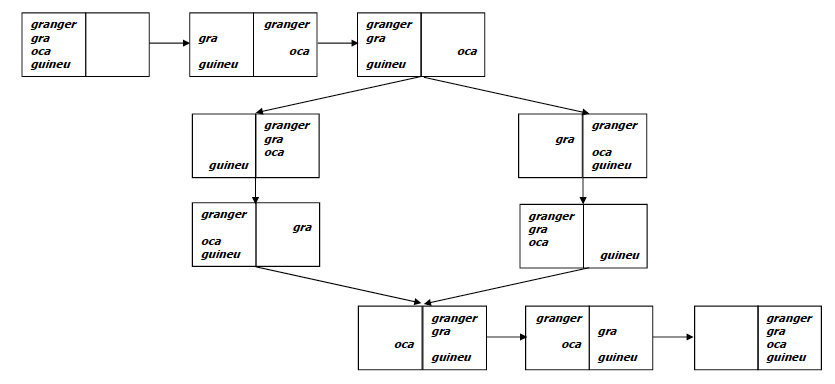
\includegraphics[width=7.57in,height=3.48in]{./media/image4.png}
\end{figure}


%%%%%%%%%%%%%%%%%%%% Figure/Image No: 4 Ends here %%%%%%%%%%%%%%%%%%%%

\par


\vspace{\baselineskip}
\begin{justify}
\footnote{ He comptat amb l’ajuda de la Dra. Maria Vanrell,\ professora d’Intel$ \cdot $ ligència Artificial de l’Escola d’Enginyeria de la UAB, m’ha cedit  aquest cas que és el que ella mateixa usa per explicar als alumnes com funcionen els arbres de decisió en les xarxes neuronals. } {\fontsize{10pt}{12.0pt}\selectfont Veure peu de pàgina. \par}
\end{justify}\par


\vspace{\baselineskip}

\vspace{\baselineskip}
\begin{justify}
L’exemple té un principi bàsic de funcionament serà sempre el camí més òptim aquell que comporti menys passos o graus per arribar a la solució final i que aquest sigui factible, és a dir, persegueixi l’objectiu i no entomi cap camí contrari o impossibilitant d’aquest interès. He cregut convenient aportar aquest exemple per tancar el capítol tècnic perquè és molt pedagògic i fàcil d’entendre per a persones no versades en la matèria sobre el funcionament mínim de la intel$ \cdot $ ligència artificial.
\end{justify}\par

\begin{Center}
{\fontsize{16pt}{19.2pt}\selectfont \textbf{CAPÍTOL III: REGULACIÓ PATENTS}\par}
\end{Center}\par


\vspace{\baselineskip}
\begin{justify}
Aquest capítol té com a principal propòsit analitzar la regulació legal de les patents a España, Europa Estats Units. Després integrar-la i adaptar-la a la intel$ \cdot $ ligència artificial per comprovar si l’IA té un bon encaix amb la normativa actual o en tal cas si serien necessàries algunes modificacions legals. 
\end{justify}\par


\vspace{\baselineskip}
\begin{justify}
\textbf{3.1.- CONCEPTE DE PATENT}
\end{justify}\par


\vspace{\baselineskip}
\begin{justify}
El Manual de la Propietat Industrial del Professor Fernández-Nóvoa proposa la següent definició per a patent $``$\textit{la invención como una creación intelectual consistente en una regla para el obrar humano técnico, no conocida, que indica un modo no evidente de actuación de determinados medios sobre las fuerzas de la Naturaleza y de cuya actuación deriva un resultado directamente aplicable en la industria$"$ \footnote{ Fernández-Novoa, C., Otero, J.M. y Botana, M. (2017). $``$Manual de la Propiedad Intelectual. Tercera Edición$"$ . Madrid: Marcial Pons. Pàg. 114. }. } S’assimila el concepte d’invenció com el de regla, es a dir, la patent és un procediment mecànic constant que aconsegueix un resultat concret i específic seguint uns passos determinats per la pròpia tècnica amb caràcter repetitiu. Doncs bé, aquesta regla ha de ser nova, no evident i ha de ser aplicable\ directament  a la realitat.  
\end{justify}\par


\vspace{\baselineskip}
\begin{justify}
La LP en l’article 4.1 considera que $``$\textit{son patentables, en todos los campos de la tecnología, las invenciones que sean nuevas, impliquen actividad inventiva y sean susceptibles de aplicación industrial.$"$ }. Per la seva banda, el Conveni Europeu de la Patent de 1973 en l’article 52.1 considera que $``$\textit{european patents shall be granted for any inventions, in all fields of technology, provided that they are new, involve an inventive step and are susceptible of industrial application$"$ . }No hi ha quasi bé cap diferencia entre ambdues regulacions sobre quins requisits han de tenir les invencions patentables, ambdues normes recullen els requisits sobre novetat, activitat inventiva i aplicació industrial. 
\end{justify}\par


\vspace{\baselineskip}
\begin{justify}
És diferent el contingut del paràgraf 100 del Títol 35 de l’U.S.C que disposa que seran invencions patentables $``$\textit{whoever invents or discovers any new and useful process, machine, manufacture, or composition of matter, or any new and useful improvement thereof, may obtain a patent therefor, subject to the conditions and requirements of this title$"$ .} Fa un llistat de què pot ser patentat, en aquest cas processos, màquines, composicions o les seves millores si son noves i útils. No específica la qüestió de l’activitat mental de crear o el concepte d’aplicabilitat, que com veurem son de creació jurisprudencial\ als Estats Units.  
\end{justify}\par


\vspace{\baselineskip}
\textbf{1.- Idoneïtat }\par


\vspace{\baselineskip}
\begin{justify}
No totes les creacions fetes per l’ésser humà poden acomodar-se dins de la protecció jurídica de la patent, s’ha de valorar la idoneïtat cas per a cas. La pròpia LP fa un recull en l’article 4.4. d’algunes creacions que no tindran la consideració d’invencions: \textit{$``$No se considerarán invenciones en el sentido de los apartados anteriores, en particular: a) Los descubrimientos, las teorías científicas y los métodos matemáticos. b) Las obras literarias, artísticas o cualquier otra creación estética, así como las obras científicas. c) Los planes, reglas y métodos para el ejercicio de actividades intelectuales, para juegos o para actividades económico-comerciales, así como los programas de ordenadores. d) Las formas de presentar informaciones.$"$ }. Es descarta la seva adhesió a priori com a patents, perquè están mancades de tècnica, però si per algun supòsit s’afegís una part no tècnica a una altra part de caràcter tècnic s’hauria d’analitzar la naturalesa pròpia de la invenció, perquè si la part tècnica acomplís tots els requisits hauria de rebre la protecció com a patent\footnote{ Fernández-Novoa, C., Otero, J.M. y Botana, M. (2017). $``$Manual de la Propiedad Intelectual. Tercera Edición$"$ . Madrid: Marcial Pons. Pàg. 115. }. 
\end{justify}\par


\vspace{\baselineskip}
\begin{justify}
Tanmateix, l’EPC en el seu article 52.2 recull un seguit de creacions, bàsicament les mateixes que l’LP, que no rebran la consideració de patent \textit{$``$(a) discoveries, scientific theories and mathematical methods;  (b) aesthetic creations;  (c) schemes, rules and methods for performing mental acts, playing games or doing business, and programs for computers;  (d) presentations of information}{\fontsize{11pt}{13.2pt}\selectfont \textit{$"$ . }Aquests llistats no son \par}\textit{numerus clausus}{\fontsize{11pt}{13.2pt}\selectfont , sinó que poden existir altres creacions que no s’hi adeqüin per falta de requisits o per la seva naturalesa inventiva. El que és realment important en l’àmbit de la propietat industrial, és que s’evitin apriorismes i que es faci un anàlisi cas per a cas sobre la idoneïtat la invenció. \par}
\end{justify}\par

\begin{justify}
{\fontsize{11pt}{13.2pt}\selectfont En el cas dels Estats Units, el paràgraf 101 del Títol 35 U.S.C fa una discriminació positiva, selecciona quin tipus d’invenció sí que serà objecte de patent. En aquest cas, només ho podrà ser un procés, màquina, manufactura o composició de matèria, cap altre creació serà protegida com a patent sinó pertany a la numeració anterior, encara que compleixi rigorosament la resta de requisits establerts per la llei. S’ha creat a través de la jurisprudència (Sentencia Alice vs. CLS Bank International\footnote{ U.S. Supreme Court, Sentència $``$Alice vs. CLS Bank International$"$  de 19 de juny de 2014.  }), una llista jurisprudencial de discriminació negativa composada per 3 casos que no poden ser objecte de patent que son les lleis abstractes, les lleis de la naturalesa i els fenòmens naturals. Aquesta sentencia era necessària per a determinar totes les matèries que son o no idònies en el dret de propietat industrial estatunidenc. A\par}ixí doncs un cop havent analitzat què pot ser objecte de patent (\textit{subject matter eligibility)} i observant que les màquines poden produir resultats idonis de ser protegits com a patents en les 3 jurisdiccions analitzades és imperatiu examinar els requisits individualment. 
\end{justify}\par


\vspace{\baselineskip}
\textbf{2.- Novetat}\par


\vspace{\baselineskip}
\begin{justify}
En el cas espanyol, es considera que una invenció és nova quan \textit{$``$no està incluida en el estado de la técnica$"$ \footnote{ Article 6.1 de la Llei de Patents (24/2015): "Se considera que una invención es nueva cuando no está comprendida en el estado de la técnica$"$ .  }. }La novetat en les patents és un concepte de creació legal, perquè el seu contingut és el que li atorga la llei i no la que li podria conferir el propi llenguatge\footnote{ Fernández-Novoa, C., Otero, J.M. y Botana, M. (2017). $``$Manual de la Propiedad Intelectual. Tercera Edición$"$ . Madrid: Marcial Pons. Pàg. 118.  }. La novetat està vinculada amb l’estat de la tècnica actual i no amb la persona del creador. Tot allò que estigui inclòs en l’estat de la tècnica no és nou i el que quedi fora si que ho serà\footnote{ Id. Pàg.119 }. Per tant, s’haurà de determinar que és l’estat de la tècnica i què la constitueix.  La LP en l’article 6.2 estableix que $``$\textit{el estado de la técnica está constituido por todo lo que antes de la fecha de presentación de la solicitud de patente se ha hecho accesible al público en España o en el extranjero por una descripción escrita u oral, por una utilización o por cualquier otro medio$"$ . }
\end{justify}\par

\begin{justify}
L’ estat de la tècnica és universal, ultraterritorial i sense cap tipus de límit temporal. 
\end{justify}\par


\vspace{\baselineskip}
\begin{justify}
S’ha d’analitzar que s’entén pel concepte de \textit{$``$todo$"$ .} Cada sol$ \cdot $ licitud de patent haurà de ser analitzada segons la seva naturalesa. Per a decidir si una invenció està inclosa o no en l’estat de la tècnica, s’ha de comprovar si un expert amb l’estat de la tècnica actual podria reproduir-ho, en cas negatiu, no es podrà denegar la patent en base a la manca de novetat\footnote{ Id. Pàg. 120. }.  Per a determinar què composava l’estat de la tècnica abans de la presentació, s’ha d’analitzar quina informació científic-tècnica estava a l’abast del públic. S’entén com a públic qualsevol persona tercera, que sense trencar cap deure de confidencialitat o secret empresarial en tingués coneixemtn.\ Si\ l’accés hagués estat possible es consideraria com a pertanyent a l’estat de la tècnica i per tant, no se li atribuiria la condició de patent.   Per tant, la novetat ha de ser \textit{única, completa i certa\footnote{ Id. Pàg. 123. }}.  
\end{justify}\par


\vspace{\baselineskip}
\begin{justify}
L’EPC defineix que s’ha d’entendre per estat de la tècnica en l’article 54.1 \textit{$``$everything made available to the public by means of a written or oral description, by use, or in any other way, before the date of filing of the European patent application$"$ , }tampoc hi ha límits temporals o geogràfics. L’EPO ha establert alguns criteris per analitzar la informació pública que conforma l’estat de la tècnica. El primer és que tots els elements s’han d’analitzar aïlladament, el segon, és que només s’ha de tenir en compte el que expressament s’hi digui i per últim, que l’anàlisi hagi es faci des del punt de vista d’un expert\footnote{ Id. Pàg 123.  }. Per tant, si hi hagués un document que es cregués ha de ser part de l’estat de la tècnica, s’ha d’analitzar estricament el seu contingut sense relacionar-lo amb altres del mateix context temporal i fent-ho com ho hagués fet un expert en la matèria. 
\end{justify}\par


\vspace{\baselineskip}
\begin{justify}
El paràgraf 102 del Títol 35 sobre Patents dels Estats Units, recull totes les causes per les quals s’ha de rebutjar la concessió d’una patent per falta de novetat. El primer motiu de denegació és que la patent ja sigui coneguda a altra països, o per suposat patentada. El segon motiu seria l’abandonament de la invenció. El tercer motiu és que la invenció hagués estat descrita en una publicació o com a part en altres patents. El tercer motiu és que el sol$ \cdot $ licitant no hagués inventat la creació per la qual està demanant la patent. El quart motiu, es que algú hagués demanat abans la protecció en un altre país tenint en compte la data de sol$ \cdot $ licitud. Aquest llistat exhaustiu, difereix de la generalitat continguda en el dret continental que planteja només la inserció o no en l’estat de la tècnica per a determinar la novetat o no de la creació. El que és clar, nogensmenys, el requisit de novetat s’exigeix en totes les jurisdiccions amb les diferents variants i requisits. 
\end{justify}\par


\vspace{\baselineskip}
\textbf{3.- Activitat inventiva}\par


\vspace{\baselineskip}
La patent no només ha de ser idònia i novedosa, sinó que ha de suposar activitat inventiva al menys per la LP. L’article 8.1. assenyala que $``$\textit{se considera que una invención implica una actividad inventiva si aquélla no resulta del estado de la técnica de una manera evidente para un experto en la materia$"$ . }Si la invenció fos resultat d’una combinació obvia de l’estat de la tècnica, estaria directament mancada d’activitat inventiva. No vol dir això que sigui imperatiu que el creador millori l’estat de la tècnica, sinó que la seva creació hagi resultat d’un procés innovador i disruptiu sobre el coneixement actual i no previsible. \par


\vspace{\baselineskip}
L’examen de l’activitat inventiva ha de ser el màxim objectiva perquè ha de vincular-se amb la definició de l’estat de la tècnica i el coneixement mig d’un expert en la matèria en aquell moment temporal concret. Aquest examen es duu a terme seguint el mètode de $``$\textit{problem and solution approach$"$ \footnote{ European Patent Office. $``$Guidelines for examination: Problem-Solution Approach$"$ . Recuperat de [05/02/2020]: https://www.epo.org/law-practice/legal-texts/html/guidelines/e/g\_vii\_5.htm }}, que pretén fonamentalment evitar una valoració de la activitat inventiva \textit{ex post facto, }amb el que es tracta de donar major objectivitat a l’anàlisi d’obvietat en la data en la que es reivindica. El funcionament del paradigma és el següent, primer es determina l’estat de la tècnica, el segon pas és definir quina solució aporta la invenció i per últim, tenint en compte els dos elements anteriors, valorar si la invenció era o no evident als ulls d’un expert\footnote{ Asensi, A., García, A., Gimeno, V. et al. (2019) $``$Reseña de actualidad: Propiedad intelectual$"$ . Alicante: La Ley Mercantil, núm. 61.  }. \par

L’expert és una persona que ha de tenir els coneixements propis del seu camp de professió, es tracta d’una persona que es troba actualitzada en les novetats del seu camp i te les eines per a cercar tota la informació per definir l’estat de la tècnica. Aquest expert haurà de determinar si l’extracció del raonament per a crear la invenció era evident. La determinació del que és evident és el repte, perquè dependrà de quin grau d’obvietat s’accepti per part dels examinadors.  \par


\vspace{\baselineskip}
El requisit de l’activitat inventiva és el més arbitrari i inconcret de tots perquè dependrà d’una decisió subjectiva d’on posem els límits de que entenem per activitat inventiva tenint en compte l’explicat, com que els tribunals han estat conscients de la dificultat i complicació en els exàmens a l’OPEM però també a l’EPO, la jurisprudència ha assenyalat algunes característiques s’han tenir en compte per a determinar s’hi ha activitat inventiva. El Manual de la Propietat Industrial relaciona els següents, la importància de la pròpia invenció, els avantatges nous  i imprevistos, la solució d’un problema llargament plantejat, l’èxit comercial degut a la naturalesa del producte, la superació d’algun prejudici tècnic, l’aportació que suposa la invenció en un camp específic, la simplicitat de la solució donada a un problema complex, entre d’altres que poden utilitzar per a validar l’activitat inventiva\footnote{ Fernández-Novoa, C., Otero, J.M. y Botana, M. (2017). $``$Manual de la Propiedad Intelectual. Tercera Edición$"$ . Madrid: Marcial Pons. Pàg. 11. }. \par


\vspace{\baselineskip}
Als Estats Units, el concepte que s’usa és el de $``$\textit{non-obvious subject matter$"$  }recollit al paràgraf 103 del 35 U.S.C que s’equipara al dret continental, en el sentit de que la invenció no ha de ser obvia en relació amb l’estat de la tècnica en el moment temporal concret. Per a determinar-ho s’usa el mesurador anomenat PHOSTIA (\textit{Person having ordinary skill in the art)\footnote{ Abbott, R. (2016). $``$I think, therefore I invent: Creative Computers and the Future of Patent Law$"$ . EE.UU.: Boston College Law Review. Pàg. 1124. }}, es presumirà quin és el coneixement mitjà d’una persona entesa en el camp concret de la invenció, com en el cas del dret continental i l’expert, per a determinar la obvietat o no de la invenció. \par


\vspace{\baselineskip}
L’examinador un cop rebuda la sol$ \cdot $ licitud la compararà amb les patents més pròximes al camp tècnic concret de la invenció, per a comprovar si combinant pocs elements la invenció és possible, si això passés s’hauria de rebutjar la creació com a patentable. Aquest procediment és va crear jurisprudencialment en la Sentencia KSR International Co v. Telefex Inc\footnote{ U.S. Supreme Court. Sentència $``$KSR International Co v. Telefex Inc.$"$  de 30 d’abril de 2007 }, on el Tribunal Suprem va considerar que només amb dues referencies  de patents pròximes a la invenció es produïa un resultat previsible, no hi havia cap novetat en la seva combinació, encara que no hi hagués hagut cap pista prèvia i pública de que eren combinables. Com en el dret continental, els tribunals han procurat clarificar el requisit sobre l’activitat inventiva que és el més conflictiu. \par


\vspace{\baselineskip}
Tant en el dret continental com en el dret anglosaxó s’ha objectivitat la determinació de la obvietat desvinculant-ho de la persona del inventor, no es té en compte els seus coneixements previs ni es valora si hi hagut un procediment mental o no. Es valora sobre el coneixement previ i sobre la probabilitat de aconseguir un resultat concret sense afegir-hi creativitat pròpia del expert. És molt rellevant aquest punt perquè aquest paradigma és aplicable a l’IA, on l’important és l’anàlisi del resultat i no la figura del creador o els coneixements previs que en tingués sinó que el resultat pot quedar fora de l’estat de la tècnica per un PHOSTIA.\par


\vspace{\baselineskip}
\textbf{4.- Aplicabilitat}\par


\vspace{\baselineskip}
\begin{justify}
La LP considera una invenció com a patentable sempre que sigui possible aplicar-la en la industria, l’article 9.1 estableix que $``$\textit{se considera que una invención es susceptible de aplicación industrial cuando su objeto puede ser fabricado o utilizado en cualquier clase de industria, incluida la agrícola$"$ .} Per tant, serà d’aplicació si es pot fabricar, es a dir, transformar en producte o si es pot introduir en el procés de fabricació, podent ser patentable el propi procés.\  L’ EPC estableix exactament el mateix contingut que la LP, en l’article 57 considerant que $``$\textit{an invention shall be considered as susceptible of industrial application if it can be made or used in any kind of industry, including agriculture". }El cas del Estats Units és diferent perquè la llei només diu que ha de ser útil\footnote{ Títol 35 U.S.C 101 Inventions patentable. $``$Whoever invents or discovers any new and useful process, machine, manufacture, or composition of matter, or any new and useful improvement thereof, may obtain a patent therefor, subject to the conditions and requirements of this title$"$ .  } però no concreta si ha de ser fabricat o usat, només que ha de tenir una utilitat pràctica, en aquest sentit, tampoc hi ha una obligació de que sigui a la indústria com a tal sinó que potser de qualsevol sector sempre i quan tingui un propòsit funcional. 
\end{justify}\par


\vspace{\baselineskip}
\begin{justify}
\textbf{3.2.- AUTORIA }
\end{justify}\par


\vspace{\baselineskip}
\begin{justify}
Aquest epígraf que ens ocupa versarà únicament sobre la normativa sobre qui és l’autor en les diferents jurisdiccions, en el Capítol IV serà quan s’explicaran altres models alternatius amb la variable nova de l’IA però per arribar a tal objectiu és imprescindible conèixer la normativa actual d’atribució de l’autoria de les invencions.  La LP en l’article 10.1 estableix que \textit{$``$el derecho a la patente pertenece al inventor o a sus causahabientes y es transmisible por todos los medios que el derecho reconoce$"$ }, es a dir, serà reconegut com a propietari l’inventor i els seus hereus. En els casos on hi hagi més d’un autor $``$\textit{el derecho a obtener la patente pertenecerá en común a todas ellas\footnote{ Llei de Patents, 24/2015, de 24 de juliol. Article 10.2 $``$Si la invención hubiere sido realizada por varias personas conjuntamente, el derecho a obtener la patente pertenecerá en común a todas ellas$"$ . }$"$ } segons previst en l’article 10.2 de la LP. 
\end{justify}\par


\vspace{\baselineskip}
\begin{justify}
L’article 60 de l’EPC reprodueix el mateix contingut que l’article 10 de la LP, diu així $``$\textit{1. The right to a European patent shall belong to the inventor or his successor in title [...]. }Per tant, se li atorgarà el dret a la propietat a l’inventor o en el seu cas, hereus. En el cas dels Estats Units el paràgraf 115, Títol 35 del U.S.C, estableix que el sol$ \cdot $ licitant haurà de ser aquell que cregui ser el primer inventor d’un procés, màquina, manufactura, composició de matèria, o de les seves millores, per la qual sol$ \cdot $ licita la patent. Per tant, estarà legitimada aquella persona que cregui que és el primer. En el cas de que hi hagi més de dos inventors, hauran de sol$ \cdot $ licitar la patent de forma conjunta\footnote{ Títol 35 U.S.C 116 Inventors: $``$When an invention is made by two or more persons jointly, they shall apply for patent jointly and each make the required oath, except as otherwise provided in this title. Inventors may apply for a patent jointly even though (1) they did not physically work together or at the same time, (2) each did not make the same type or amount of contribution, or (3) each did not make a contribution to the subject matter of every claim of the patent$"$ . }.  En les tres jurisdiccions hi ha el principi de prioritat, tindrà preferència sempre per a obtenir el dret a la patent la persona que hagués presentat abans la sol$ \cdot $ licitud d’obtenció, seguint el principi general del dret $``$\textit{prior in tempore, potior in iure$"$ . }És comuna, també, l’atribució dels dret de propietat en la persona de l’inventor.
\end{justify}\par


\vspace{\baselineskip}
\begin{justify}
\textbf{3.3.- INTEGRACIÓ DE L’IA EN LA NORMATIVA DE LES PATENTS}
\end{justify}\par


\vspace{\baselineskip}
\begin{justify}
Per a abordar aquest paràgraf el més convenient és fer-ho a través d’un exemple creat per l’IA i anar fer la seva adaptació als requisits normatius de les patents que s’han analitzat en aquest Capítol. 
\end{justify}\par


\vspace{\baselineskip}
\begin{justify}
He escollit les receptes de cuina produïdes per Watson que hem explicat en el Capítol II com a objecte d’anàlisi perquè ja hem conegut el seu funcionament i alguns exemples tradicionals de receptes que han estat patentades.  Les receptes creades per Watson es basaven en informació que li introduïen els usuaris, en cap cas, eren fórmules culinàries sinó aliments, tipologies de cuina, etc. El resultat de les creacions de Watson es van incloure en un llibre anomenat \textit{$``$Cognitive Cooking with Chef Watson: Recipes for innovation from IBM $\&$  THE Institute Of Culinary Education$"$ \footnote{ IBM $\&$  Institute of Culinary Education (2015) $``$Cognitive Cooking with Chef Waston: Recipes for innovation from IBM $\&$  THE Institute Of Culinary Education$"$ . EE.UU.: Sourcebooks }, }he seleccionat una de les receptes que inclou el llibre per a poder analitzar-la segons els\ requisits normatius  de les patents que s’han exposat i veure quin encaix hi podria tenir, és una ficció però pot exemplificar molt bé la conjunció entre producte creat per IA i la seva patentabilitat. La recepta s’anomena $``$Indian Turmeric Paella$"$ \footnote{ Id. Pàg 26 – 27. }, és a dir, Paella Índia de Cúrcuma. En un inici, no hi ha cap contradicció aparent amb l’article 4.4 de la LP, el 52.2 de l’EPC o el paràgraf 101 del 35 U.S.C., aquesta recepta presenta la condició d’idoneïtat per a ser patentada perquè no està inclosa en cap excepció normativa del dret continental i està prevista en la Llei de Patents del Estats Units com a composició de matèria. 
\end{justify}\par


\vspace{\baselineskip}
\begin{justify}
El segon requisit és que inclogui un factor de novetat. En aquest cas, s’hauria de conèixer en profunditat l’estat de la tècnica concreta en el moment de la seva creació, doncs així podríem determinar si la combinació d’ingredients estava inclosa com a coneixement general públic. Per tant, tot i no poder assegurar la seva novetat perquè no tenim el coneixement tècnic culinari, podem dir que tampoc sembla difícil que aquesta recepta fos única en l’estat de la tècnica, podríem fer un apriorisme d’encaix positiu.
\end{justify}\par


\vspace{\baselineskip}
\begin{justify}
El tercer requisit és que hi hagi una activitat inventiva. Per a determinar-la és necessari definir si el resultat podia ser obvi o no a ulls d’un expert. El cert és que la recepta té més de 21 ingredients\footnote{ Id. Pàg 26 – 27. } que no son els propis de la Paella que coneixem com per exemple, els tomàquets xerri, la cúrcuma o el fonoll. En aparença, la combinació podria no ser obvia per un expert culinari i per tant, que Watson hagi inventat una combinació que no era previsible als ulls d’un expert cuiner.
\end{justify}\par


\vspace{\baselineskip}
\begin{justify}
Per últim, hi ha el requisit de la aplicabilitat en la indústria, doncs bé, es podria usar per part de qualsevol empresa que produís menjar precuinat o en serveis d’hostaleria, així que compliria amb el requisit d’utilitat i aplicabilitat.  
\end{justify}\par


\vspace{\baselineskip}
\begin{justify}
Podem preveure que no hi ha dificultats aparents, sense entrar en l’examen profund del cas concret, que aquesta recepta acomplís els requisits de la protecció jurídica de la patent\footnote{ Deixant de costat la seva possible admissió real o no per les diferents Oficines de Patents i Marques. És un exemple pràctic per fer l’encaix de la qüestió.  }. Per tant, en tot cas, la creació realitzada a través de l’IA podria ser patentable tenint en compte els requisits legals que estableixen les lleis.La dificultat sorgiria si volguéssim sol$ \cdot $ licitar-ne la patent, perquè l’inventor en termes d’estricta realitat, és una xarxa neuronal anomenada Watson, com hem vist, el dret continental com l’anglosaxó, preveuen a persones físiques com a inventors, ergo, legitimades per a obtenir els drets sobre la invenció. 
\end{justify}\par

\begin{justify}
L’ any 2019, l’ $``$Artificial Inventor Project$"$  \footnote{ És una organització que fa recerca prospectiva sobre drets de propietat intel$ \cdot $ lectual e industrial producte de la Intel$ \cdot $ ligència Artificial. Recuperat de [05/01/2020]: http://artificialinventor.com/ } va sol$ \cdot $ licitar els drets de patent per a dos productes creats per una Intel$ \cdot $ ligència Artificial davant de l’EPO. L’EPO va rebutjar patentar les dues sol$ \cdot $ licituds\footnote{ European Patent Register. (2019). Sol$ \cdot $ licitud núm. EP 18 275 163 i núm. EP 18 275 174. Recuperat de [05/01/2020]: https://register.epo.org/application?number=EP18275174 https://register.epo.org/application?number=EP18275163 } en base als articles 81 i Regla 19 del EPC, que assenyalen el següent $``$\textit{la designació del inventor haurà d’efectuar-se en la sol$ \cdot $ licitud de concessió de patent europea. No obstant, si el sol$ \cdot $ licitant no fos l’inventor o l’únic inventor, la menció haurà de realitzar-se en un document presentat per separat, en el que hauran de recollir el cognom el nom i la direcció completa del inventor$"$ . }El que va al$ \cdot $ legar l’EPO com a resposta a les sol$ \cdot $ licituds es que el requisit de determinar el cognom, nom i direcció no és un mer formalisme i que està intimament lligat al fet de tenir personalitat, perquè per exercir el drets que se li reconeixen és essencial que sigui una persona física i que per tant, una màquina no podia ser reconeguda com a inventora\footnote{ Zafrilla, V. (2020). $``$Caso DABUS: la EPO rechaza que la AI pueda ser designada como inventor de una patente$"$ . Recuperat de [08/01/2020]: http://www.lvcentinvs.es/2020/01/30/caso-dabus-la-epo-rechaza-que-la-ai-pueda-ser-designada-como-inventor-de-una-patente/ }. El que entra en contradicció absoluta amb l’ article 60 del EPC que estableix $``$\textit{el dret a la patent europea pertany a l’inventor o els seus hereus$"$ }, per tant, si l’inventor és una màquina i no se la reconeix com a tal, no s’estaria inaplicant la llei?  
\end{justify}\par

\begin{justify}
Si les invencions computacionals compleixen els requisits de patentabilitat, però l’IA no pot ser reconeguda com a inventora suposa que la primera persona que s’adoni de la creació de la invenció com a tal seria la legitimada per a considerar-se inventora i propietària dels drets\footnote{ Abbott, R. (2016). $``$I think, therefore I invent: Creative Computers and the Future of Patent Law$"$ . EE.UU.: Boston College Law Review. Pàg. 1116. }. Això suposaria greus distorsions perquè podria ser reconeguda com a inventora una persona que no hagi aportat cap contribució conceptual o creativa a la invenció i que només s’hagi adonat de les condicions de patentabilitat de la creació\footnote{ Chimuka, G. (2019). $``$Impact of Artificial Intelligence on Patent Law. Towards a new analytical framework [The Multi-Level Model]$"$ , U.K.: World Patent Information, núm.59. Pàg. 8. }. És necessari analitzar altres models que ha proposat la literatura sobre l’autoria i la propietats de les patents creades a través de l’IA. 
\end{justify}\par

\begin{Center}
{\fontsize{16pt}{19.2pt}\selectfont \textbf{CAPÍTOL IV: AUTORIA COMPUTACIONAL}\par}
\end{Center}\par


\vspace{\baselineskip}
\begin{justify}
Aquest capítol és una vista panoràmica de les aproximacions més rellevants que s’han elaborat per la literatura especialitzada, majoritàriament nord-americana, per a donar resposta a la casuística entre la dicotomia autor i propietari de les patents en l’era de l’IA. El paradigma tradicional de la les diferents normatives sobre patents son inaplicables i ineficients davant dels reptes que els canvis tecnològics ens plantegen i per les quals s’han de buscar diferents solucions. La majoria de propostes es fonamenten en el principi de separació d’autoria i de la propietat, modificant la normativa actual on hi ha un automatisme entre la figura de l’autor i la del propietari. 
\end{justify}\par


\vspace{\baselineskip}
\begin{justify}
\textbf{4.1.- AUTORIA}
\end{justify}\par


\vspace{\baselineskip}

\vspace{\baselineskip}
\begin{justify}
Davant dels resultats creats per la intel$ \cdot $ ligència artificial hi ha tres propostes principals de literatura per assignar-ne l’autoria seguint diferents criteris jurídics, algunes\ de més  conservadores i altres de més reformistes. Tant la teoria de l’autor-persona com del domini públic, son propostes que inclouen en el seu sí la propietat. 
\end{justify}\par


\vspace{\baselineskip}
\textbf{1.- Autor-persona}\par


\vspace{\baselineskip}
\begin{justify}
L’aproximació inicial més senzilla és aquella que proposa que l’autoria s’ha d’atribuir a l’ésser humà que hi ha darrere de la màquina, aquesta és la solució\footnote{ Copyright, Designs and Patents Act. (1988). Section 9(3): $``$In the case of a literary, dramatic, musical or artistic work which is computer‐generated, the author shall be taken to be the person by whom the arrangements necessary for the creation of the work are undertaken$"$ . } que  ha regulat el Regne Unit que son juntament amb l’Índia, els únics dos països que han positivitzat la creació realitzada per ordinadors sobretot en l’àmbit de la propietat intel$ \cdot $ lectual. Sorgeix un problema principalment en l´ús pràctic d’aquest paradigma, que és identificar clarament qui és la persona que es troba darrere de la màquina. Hi ha multitud de participants en la construcció i posada en marxa de la xarxa neuronal, trobem programadors, usuaris, proveïdors de dades o inversors, determinar qui de totes les persones ha estat la més determinant en aconseguir el resultat és quasi bé impossible.
\end{justify}\par


\vspace{\baselineskip}
\begin{justify}
Per il$ \cdot $ lustrar-ho millor és necessari presentar un exemple, l’any 2019 es va subhastar un quadre anomenat $``$Edmond de Belamy$"$  per 380.000 euros a través de la famosa casa de subhastes Christie’s. Darrere del quadre hi havia 3 amics de Paris que van utilitzar una xarxa neuronal de codi obert que havia creat el projecte de Xarxes Generatives Antagòniques\footnote{ Núñez, N. (2019) $``$El primer cuadro de inteligencia artificial, vendido por Christie’s$"$ .El PAIS. Recuperat de [08/12/2019$"$ : https://elfuturoesapasionante.elpais.com/el-primer-cuadro-de-inteligencia-artificial-vendido-por-christies/ } introduint-hi milers d’imatges per a crear una obra totalment nova i original. Es va suscitar una gran polèmica sobre s’hi el creador de la xarxa neuronal havia de rebre part del premi per haver contribuït amb l’eina, però va ser fàcil de concloure que seguint la teoria de l’autor persona l’aportació significativa va ser dels 3 amics parisencs que van introduir, seleccionar, modificar i entrenar l’IA per aconseguir el resultat final. En aquest cas, la teoria de l’autor-persona és fàcilment aplicable perquè definir qui va ser  l’autor darrere de la màquina és relativament senzill perquè hi havia pocs actors en el cas i perquè van fer una aportació significativa per aconseguir aquell determinat resultat.  
\end{justify}\par


\vspace{\baselineskip}
\begin{justify}
Hi ha casos que no son tant clars, on aquesta teoria és inaplicable o en el seu cas, s’aplicaria en frau de llei o de manera incoherent. Imaginem un periodista que introdueix algunes dades històriques, molt minses, sobre els faraons a Egipte i amb aquesta poca informació, la màquina crea un article extens sobre la temàtica. Seria èticament just o en el seu cas, legal, l’atribució de l’autoria al periodista\footnote{ López-Tarruella, A. $``$¿Pueden las maquinas ser consideradas autores?$"$  España: Revista Telos. Núm 112. Pàg 125-129.  }? Semblaria que no \textit{a priori}, ja que el sistema de drets d’autor està estructurat per recompensar l’esforç intel$ \cdot $ lectual de l’autor protegint-ne l’obra, passa exactament igual que amb la propietat industrial on és recompensa l’activitat inventiva i en aquest cas, és clar, que no n’hi hagut. Per tant el sistema de protecció es faria en frau de llei perquè l’autor no ha inventat o creat el resultat. S’hauria de diferenciar entre aquelles invencions creades a través d’una aportació significativa de l’esser humà i aquelles on no s’ha produït cap aportació ressenyable, perquè sinó estaríem recompensant esforços intel$ \cdot $ lectuals inexistents i seria un sistema totalment ineficient i fraudulent, i per tant, deslegitimat. 
\end{justify}\par


\vspace{\baselineskip}
\begin{justify}
Aquest paradigma té un segon problema, si l’atribució sobre l’autoria s’hagués de fer a una persona física, ens trobaríem que se li podria atribuir a la primera persona que reconegués la invenció com a patentable i la registrés. Per exemple, en un paradigma tradicional, si una persona crea una bateria millorada per l’Iphone, aquesta persona sempre serà l’autora encara que algú altre se’n adoni o no i ningú més s’ho podria atribuir com a propi. Però en el paradigma actual de creacions a través de màquines, si aquesta persona no ho ha creat sinó que ho ha fet una màquina, la primera persona en adonar-se’n i reconèixer-ho seria l’inventor en termes legals\footnote{ Abbott, R. (2016). $``$I think, therefore I invent: Creative Computers and the Future of Patent Law$"$ . USA: Boston College Law Review. Pàg. 1104. }. Aquesta possibilitat obriria la porta a que persones que no estiguessin relacionades amb la creació o amb la màquina, poguessin atribuir-se’n els drets sobre la mateixa
\end{justify}\par


\vspace{\baselineskip}
\begin{justify}
Aquest aproximació on l’autor és la persona, és la\ que te un major encaix amb les lleis actuals perquè reconeixen l’autor com una persona  i per tant, li atribueix els drets que se’n deriven, com ja està previst actualment per totes les invencions. Però és ineficient per afrontar els reptes que els canvis tecnològics estan ja suposant perquè donaria l’oportunitat en molts dels casos, una aplicació incoherent i fraudulenta dels drets.
\end{justify}\par


\vspace{\baselineskip}
\begin{justify}
\textbf{2.- Autor-màquina}
\end{justify}\par


\vspace{\baselineskip}
Aquesta opció és la que proposa que se li atribueixi l’autoria a la màquina. La majora de la literatura que defensa aquesta teoria, diferencia entre el reconeixement de la figura d’autor i l’assignació de la propietat sobre el drets. Aquest paradigma proposa reconèixer l’autor-màquina, quan aquesta hagi fet l’aportació principal en la creació de la invenció en detriment de la persona. \par

Aquesta proposta suposaria reformar la normativa profundament, com ja s’ha analitzat en aquesta recerca anteriorment, no hi ha cap text legal on es reconegui la possibilitat de que un autor sigui una màquina. La negativa a reconèixer la màquina com a autora per manca d’activitat inventiva, implica l’assumpció indirectament de que la intel$ \cdot $ ligència artificial no pot assimilar-se a la intel$ \cdot $ ligència humana\footnote{ López-Tarruella, A. $``$¿Pueden las maquinas ser consideradas autores?$"$  Revista Telos. Núm 112. Pàg 125-129. }, que és xocant tenint en compte els avenços científics i objectius aconseguits fins ara com s’ha explicat en el Capítol II d’aquesta recerca. Assumir que les invencions produïdes per una màquina no son igual d’originals o creatives que les pròpies d’una ment humana, suposa tancar els ulls a la realitat que estem vivint on hi ha milers d’exemples que compleixen els requisits de patentabilitat i que han estat creats exclusivament per màquines i que si s’atribuïssin a persones físiques s’estaria fent en frau de llei. \par


\vspace{\baselineskip}
Alguna part de la doctrina creu que la teoria de l’autor-màquina, suposa un problema perquè suposaria dotar a la màquina de reconeixement com a persona jurídica que tindria un impacte en el Dret Civil\footnote{ Id. }, però aquesta visió és molt determinista perquè no hi ha cap raó per assignar personalitat jurídica a la màquina, ja que no seria reconegut com a propietari ni executor dels drets, només suposaria una diferenciació de les figures per a garantir una major seguretat jurídica però en cap cas, seria necessària l’atribució de personalitat jurídica per a poder ser autor.  \par


\vspace{\baselineskip}
La doctrina favorable ho fa a través de tres arguments principals; la seguretat jurídica en el tràfic mercantil de la propietat industrial i la seva protecció. Per l’altre banda, l’opció de patentar els resultats implicaria un incentiu en la creació de màquines\footnote{ Abbott, R. (2016). $``$I think, therefore I invent: Creative Computers and the Future of Patent Law$"$ . EE.UU.: Boston College Law Review. Pàg. 1.104. } més avançades i eficients perquè per inventar les màquines no necessiten cap motivació per a crear però si que la necessiten els propis programadors, desenvolupadors, inversors, etc. Per últim, a nivell jurídic és interessant veure com el fet de proporcionar al mercat la protecció com a patents suposa la promoció del descobriment i la comercialització perquè sinó seria fàcil preveure que els interessats la mantindrien\  com a secret empresarial\footnote{ Id. }. Sense la protecció de la patent seria complicat fer la transició des de la creació fins a la comercialització amb garanties jurídiques suficients\footnote{ Com succeiria amb l’aplicació de la teoria de l’Autor-persona.  } de que el procés fos exitós i econòmicament el màxim de beneficiós per tots els actors i la societat. \par


\vspace{\baselineskip}
\textbf{3.- Domini públic}\par


\vspace{\baselineskip}
Per últim, hi ha una tercera teoria que atribueix l’autoria al domini públic. La premissa de partida és que les invencions produïdes per una màquina no poden ser originals per manca d’activitat inventiva humana, i per tant, no poden ser susceptibles de la protecció legal de les patents perquè no son coherents amb la normativa. La solució proposada és que s’inclogués en l’anomenat domini públic, suposaria que totes les invencions fossin obertes i lliures, per tant, es podrien usar per tots els particulars o per l’administració pública en múltiples circumstàncies. Alguns autors com Ralph Clifford han argumentat que $``$\textit{els treballs generats autònomament per ordinadors haurien ser al domini públic fins que els avenços tecnològics fessin possible la consciència pròpia\footnote{ Clifford, R. (1997). $``$Intellectual Property in the Era of Creative Computer Program$"$ . EE.UU.: Tulane Review núm 71. Pàg. 1702-1703. Recuperat de [20/02/2020]: https://scholarship.law.umassd.edu/cgi/viewcontent.cgi?article=1077$\&$ context=fac\_pubs }$"$  }de l’IA per a decidir que és el millor a fer amb els seus resultats (Super IA). Aquesta aproximació no es troba exempta de problemes, principalment en quant a atribucions que haurien d’estar en aquesta categoria però que ja s’ han atribuït  a persones físiques com ha passat a l’USPTO en milers d’ocasions\footnote{Abbott, R. (2016). $``$I think, therefore I invent: Creative Computers and the Future of Patent Law$"$ . EE.UU.: Boston College Law Review. Pàg. 1.090. } on invencions creades per màquines han estat objecte de la figura de la patent. Hi ha un segon factor de caràcter econòmic, si les invencions fossin gratuïtes, tenint en compte la progressió esperada de l’IA, generaria que la majoria de persones deixessin d’usar les invencions que son privades perquè de forma indirecta hauríem construït una barrera de mercat en contra dels inventors humans i en favors dels inventors màquina que acapararien tot el mercat.\par

\textbf{4.2- MODELS DE PROPIETAT}\par


\vspace{\baselineskip}
\begin{justify}
En aquest apartat s’exposen les diferents teories sobre la propietat de les patents quan l’autor és una màquina. Son propostes que ha realitzat la literatura des de diferents corrents filosòfiques i paradigmes economics, entre elles contradictòries i amb punts de vista totalment dispars però que és rellevant conèixer per a poder valorar totes les opcions,  en relació a una matèria absolutament disruptiva i innovadora. 
\end{justify}\par


\vspace{\baselineskip}
\begin{justify}
\textbf{1.- Model Multi-jugador }
\end{justify}\par


\vspace{\baselineskip}
\begin{justify}
Els autors Shlomit i Xiaoqiong en el seu $``$paper$"$ \footnote{ Shlomit i Xiaoqiong (2017). $``$When Artificial Intelligence systems produce inventions: an alternative model for Patent Law at the 3A Era$"$ . EE.UU.: Cardozo Law Review.  } fan una aproximació teòrica per a definir qui ha de ser el propietari de les invencions quan el creador és un sistema d’intel$ \cdot $ ligència artificial. Elaboren un llistat d’actors rellevants en la creació d’IA i de les seves invencions. Entre d’altres, assenyalen els següents: programadors\ de\ software, proveïdors de dades, entrenadors, propietaris del sistemes d’IA,  operadors del sistema (entesos com els distribuïdors), govern,  inversors i el propi sistema d’IA que és autònom\footnote{ Id. Pàg. 2231-2232. }. Aquests actors i la seva participació es combinen amb les 3 teories clàssiques que han servit per a justificar l’existència de les patents en el sistema jurídic nord-americà, per a arribar a un model idoni d’atribució de la propietat quan l’autor és una màquina. 
\end{justify}\par


\vspace{\baselineskip}
\begin{justify}
La primera teoria que utilitzen és la que es basa en l’utilitarisme de John Stuart Mill, el principi rector és el de $``$\textit{la màxima felicitat per al màxim número de persones}$"$ , en termes econòmics seria maximitzar el benestar social per al màxim número de persones. Aquesta teoria s’aplica en la propietat industrial  per evitar i minimitzar el fenomen dels $``$\textit{free-riders$"$ }, es a dir, tot aquell seguit de persones que no pagarien l’adequat sinó hi hagués una normativa que els obligués, perquè copiarien sense recompensar als inventors\footnote{ Id. Pàg. 2237. }. Per tant, l’objectiu principal és incentivar l’activitat inventiva atorgant els drets exclusius sobre les creacions, evitant que tercer puguin utilitzar els productes sense permís. Però també hi ha un últim objectiu, que nous dissenys i tecnologies acabin al domini públic, ja que passat el temps de protecció tots les invencions passen a ser del bé comú. Les màquines no requereixen incentius, però si que en necessiten els participants en el sistema de patents. Els autors consideren que aquesta aproximació és ineficient per analitzar qui és l’actor que hauria de ser propietari sinó que és necessari recórrer a altres teories per fer-ne l’anàlisi.
\end{justify}\par


\vspace{\baselineskip}
\begin{justify}
La segona teoria és la teoria del treball de Locke, basat en el principi de que $``$\textit{el treball de les seves mans ha de ser propietat de l’home$"$ , }així doncs l’home ha de ser el propietari dels fruits del seu treball. Aplicat a la propietat de les patents l’objectiu seria recompensar la feina realitzada per l’inventor de forma justa. El problema sorgeix quan hi ha més d’un actor que participa en el procés,  que haurien de ser recompensats segons la seva contribució des dels programadors als operadors\footnote{ Id. Pàg. 2241- 2242. } de forma proporcional. Com les seves contribucions son poc creatives i es basen en acomplir ordres de tercers, com en el cas dels programadors que realitzen la seva tasca per un mandat laboral en la majoria de casos, la teoria de Locke és insuficient perquè la seva recompensa és el propi salari, i seria de propietat de l’empresa o inversors que no han realitzat la feina, es a dir, no es recompensaria la tasca a qui l’ha fet per una qüestió de funcionament de mercat. 
\end{justify}\par


\vspace{\baselineskip}
\begin{justify}
La última teoria és de la personalitat de Hegel. El principi rector d’aquesta teoria és que \textit{$``$la idea pertany al creador perquè és una manifestació de la seva personalitat$"$ , }es a dir, l’inventor té dret natural a tot el que ha inventat\footnote{ Id. Pàg. 2244 - 2245. }. Com que l’autor és una màquina, la resta d’actors fan una activitat més tècnica i menys creativa que no implica una cessió de la seva personalitat.  
\end{justify}\par


\vspace{\baselineskip}
\begin{justify}
El autors conclouen que cap d’aquestes teories, de les que han justificat històricament l’existència de les patents, son vàlides per a assignar la propietat. No tanquen la qüestió  de l’atribució de la propietat sinó que la deixen oberta.\  Aquestes teories clàssiques que han justificat la propietat sobre les invencions son insuficients, ineficaces  i incoherents amb el nou paradigma de propietat industrial. 
\end{justify}\par


\vspace{\baselineskip}
\begin{justify}
\textbf{2.- Model per defecte}
\end{justify}\par


\vspace{\baselineskip}
\begin{justify}
Ryan Abbott, professor de la Universitat de Surrey, conscient de que un cop atribuïda l’autoria a una màquina, queda pendent per a resoldre l’atribució de la propietat. Proposa en el seu estudi\footnote{ Abbott, R. (2016). $``$I think, therefore I invent: Creative Computers and the Future of Patent Law$"$ . EE.UU.: Boston College Law Review. Pàg. 1.114. } que la propietat sigui sempre per defecte pel propietari de la xarxa neuronal perquè considera que és el més coherent pel funcionament de la propietat privada i de retruc incentiva encara més la creació de xarxes neuronals\footnote{ Id. Pàg. 1.115. } perquè els propietaris poden promoure’n l’ús.\  Si aquesta assignació és per defecte, amb posterioritat podrien establir-se altres negociacions entre els participants segons els interessos i beneficis, aquest funcionament aporta més seguretat jurídica perquè és previsible.
\end{justify}\par


\vspace{\baselineskip}
\begin{justify}
L’autor argumenta que l’assignació de la propietat a l’usuari seria ineficient. Ho fa a través del exemple de Watson on hi ha accés a la plataforma quasi bé de forma il$ \cdot $ limitada. Argumenta que si els resultats en cas de ser patentables fossin assignats als usuaris, IBM es veuria compel$ \cdot $ lida a reduir l’accés a la seva plataforma però pel contrari si el resultat fos de propietat d’IBM, hi hauria suficients motius per a negociar amb els usuaris un sistema de llicencies\footnote{ Id. Pàg. 1.115. } on poguessin aconseguir la propietat o la co-propietat de les mateixes. L’atribució al desenvolupador tampoc funcionaria perquè no hi ha forma viable que un desenvolupador pugui controlar de forma eficient totes les invencions que les seves màquines creatives han creat\footnote{ Id. Pàg. 1.116. }, tanmateix, hi hauria una desinversió per part dels possibles compradors de les xarxes que no veurien cap manera de equilibrar la seva inversió perquè no rebrien cap compensació. 
\end{justify}\par

\begin{justify}
\textbf{3.- Model econòmic: Teorema de Coase}
\end{justify}\par


\vspace{\baselineskip}
\begin{justify}
El professor de la Universitat d’Oklahoma, Michael Schuster, proposa una model basat en el teorema de Coase\footnote{ Schuster, M. (2018). $``$Artificial Intelligence and Patent Ownership$"$  EE.UU.: Washington and Lee Law Review, núm 75. Recuperat de [08/12/2019]: https://scholarlycommons.law.wlu.edu/wlulr/vol75/iss4/5 } per assignar la propietat de les patents quan s’han creat a través d’intel$ \cdot $ ligència artificial.  El Teorema de Coase afirma que la $``$\textit{riquesa es maximitza quan les transaccions entre els drets de propietat estan ben definits i els costos son zero}$"$ \footnote{ Id. Pàg. 1.967 }. Per aplicar aquest teorema a la pràctica de la propietat industrial, hi ha dos aproximacions bàsiques que s’han de resoldre prèviament. La primera és assignar els drets a la part que més els valora perquè suposarà evitar costos de transacció, l’assignació eficient serà aquella on els costos es trobin per sota dels possibles guanys, i si la assignació és a la part més interessada no hi haurà cap cost afegit des de l’inici, perquè els drets romandran en aquesta part. 
\end{justify}\par


\vspace{\baselineskip}
\begin{justify}
Quan s’aplica aquest esquema econòmic en la pràctica del dret de la propietat industrial, s’ha d’aplicar la premissa següent: els participants actius en el mercat seran els que més valoraran la patent. Cert és que sempre es pot negociar la transmissió d’un participant a un altre però l’interessant és evitar al màxim, com hem assenyalat, els costos afegits de possibles compra-ventes, lloguers, etc., perquè quants més costos afegits hi ha menys marge de guany es té.
\end{justify}\par


\vspace{\baselineskip}
\begin{justify}
Queda doncs determinar quin actor del mercat és l’indicat per ser propietari per defecte. Per l’autor la part que estarà més interessada en el resultat és l’usuari\footnote{ Id. Pàg. 1.988. } perquè està al mercat, el coneix i vol, a través d’utilitzar la tecnologia, aconseguir avantatge sobre els seus competidors, per tant, serà el més interessat en aconseguir la patent i en pagar-ne un preu raonablement elevat, ja que coneixerà la potencialitat de la creació i del seu ús.  Fins al moment, s’han exposat els principals models d’atribució de la propietat però és imperatiu per a tenir una vertadera visió holística, que s’exposi l’aproximació de caràcter obert i desregulat.
\end{justify}\par


\vspace{\baselineskip}
\begin{justify}
\textbf{4.- Model Obert}
\end{justify}\par


\vspace{\baselineskip}
\begin{justify}
Aquest model reconeix a la màquina com a inventora, a diferencia del model de domini públic on és aquest és l’autor.  El model obert advoca perquè el resultat sigui de domini públic encara que l’autor sigui una màquina. En principi, es podria creure que aquest funcionament podria desincentivar la innovació per part dels programadors o usuaris. 
\end{justify}\par


\vspace{\baselineskip}
\begin{justify}
El professor, Nick Bostrom,  de la Universitat d’Oxford defensa que hi ha un temps d’exclusivitat per a la persona que hi ha darrere de la màquina. Aquesta part té la oportunitat si és coneixedor del mercat de valorar-ne l’impacte i fer-ne un negoci lucratiu, perquè copiar o explotar un determinat àmbit de coneixement no és senzill encara que no hi hagi cap barrera legal que ho impedeixi\footnote{ Bostrom, N. (2016). $``$Strategic Implications of Openess in AI Development$"$ . U.K.: Future of Humanity Institute de la Universitat d’Oxford. Pàg. 4.  } i el resultat sigui de tota la comunitat. S’ha de tenir un cert nivell d’expertesa en un àmbit per a poder analitzar el potencial d’una creació, i aquest coneixement és relativament poc freqüent. Argumenta l’autor que la persona que hi hagi darrere de la màquina o l’ usuari tindrà un marge de explotació tot i no haver-hi cap mena de protecció legal de la invenció. Així doncs no és necessària la protecció de la invenció ni l’atribució de la propietat a cap de les parts. 
\end{justify}\par


\vspace{\baselineskip}
\begin{justify}
Aquestes teories proposen solucions dispars a través de models econòmics, sociològics i jurídics. N’hi ha que plantegen la desregulació d’aquestes invencions i l’atribució al domini públic, d’altes proposen l’atribució per defecte al propietari o a l’usuari. L’ideal serà que cada legislador operi en el seu àmbit de jurisdicció segons l’ecosistema de desenvolupament tecnològic, econòmic i social de la societat específica de que es tracti a través del model que més pugui beneficiar al comú. No obstant això, seguidament en el Capítol V proposaré el model que considero més eficient i coherent amb els reptes futurs i que sota la meva opinió pot ser objecte de millor adaptació. 
\end{justify}\par

\begin{Center}
{\fontsize{16pt}{19.2pt}\selectfont \textbf{CAPÍTOL V: PROPOSTA JURÍDICA}\par}
\end{Center}\par


\vspace{\baselineskip}
\begin{justify}
\textbf{5.- PROPOSTA}
\end{justify}\par


\vspace{\baselineskip}
\begin{justify}
Aquest estudi ha repassat en els capítols proppassats des de la part tècnica de la intel$ \cdot $ ligència artificial, la part jurídica de les patents o les propostes de la literatura davant dels nous reptes d’autoria i de propietat respecte de les invencions. Així doncs, per acabar d’aprofundir en l’estudi, he cregut convenient proposar la meva pròpia teoria davants de les transformacions tecnològiques. Sé que és agosarat definir quina regulació més idònia i optima, però després d’anys de fer prospecció en aquest camp de coneixement tant pràctic com teòric, friso per endinsar-me en la construcció d’un plantejament jurídic propi. La proposta jurídica inclou alguns aspectes que han quedat fora d’aquest estudi perquè hagués sobrepassat àmpliament l’extensió prevista pel TFG, però que és convenient detallar en aquest Capítol com per a que sigui el màxim global i que analitzi tots els àmbits que es veuen afectats. L’estructura del plantejament comença amb la regulació jurídica i econòmica de les dades, la del algorisme i per últim, l’autoria i propietat de les patents. És el cicle de creació de les invencions produïdes per intel$ \cdot $ ligència artificial i son els aspectes més importants des d’una vessant teòrica i pràctica. 
\end{justify}\par


\vspace{\baselineskip}
\textbf{1.- Dades}\par


\vspace{\baselineskip}
\begin{justify}
La Comissió Europea, l’any 2015, va predir que les dades personals dels ciutadans europeus tindrien un valor aproximat d’un bilió d’euros l’any 2020, i que el RGPD podria produir uns beneficis econòmics de 2.300 milions d’euros anuals\footnote{ European Comission. (2015) $``$Fact Sheet MEMO/15/5170$"$ . Recuperat de [4/01/2020]:  }. Tenint en compte aquestes xifres econòmiques és clara la importància que tenen les dades sobretot en el mon tecnològic. 
\end{justify}\par


\vspace{\baselineskip}
\begin{justify}
La intel$ \cdot $ ligència artificial s’alimenta de dades per a poder entrenar i millorar els seus resultats. Per tant, les dades tenen un paper fonamental en la creació de noves invencions, com s’ha vist al llarg d’aquesta recerca amb exemples com el AlphaGo! O el Chef Watson. Les dades s’han d’extreure, refinar i distribuir per a aconseguir el màxim valor possible, encara que també poden ser inútils i una càrrega\footnote{ Frank, M., Roerhrig, P. i Pring, B. (2018) $``$Qué haremos cuando las máquinas lo hagan todo: Artificial Intelligence, Bots $\&$  Big Data$"$  EE. UU.: LidSpeakers. Pàg. 87. } si no es gestionen correctament, perquè el seu ús descontrolat suposa l’assoliment de resultats confusos i una pèrdua d’eficiència, ja que provoca que les màquines hagin de treballar molt més per aconseguir resultats que siguin útils i vàlids.
\end{justify}\par


\vspace{\baselineskip}
\begin{justify}
La qüestió que es planteja és si és necessari canviar el model econòmic i jurídic actual en relació a les dades personals. Jaron Lanier, enginyer informàtic i assessor de l’UE per a qüestions tecno-ètiques, considera fonamental monetitzar les dades perquè les màquines substituiran les persones però ho faran usant la matèria prima que aquests produeixen\footnote{ Zafra, J. (2018). $``$Ser critico es el último acto de optimismo$"$ . Revista Telos, núm 109. Recuperat de [05/02/2020]: https://telos.fundaciontelefonica.com/jaron-lanier-ser-critico-es-el-ultimo-acto-de-optimismo/ }, per tant, els productors haurien de rebre una compensació econòmica. Aquí es podrien usar models com el de la personalitat de Hegel o la del treball de Locke per a justificar l’intercanvi econòmic. En aquesta línia, l’any 2015, la Unió Europea va fer un esborrany de directiva que finalment no va veure la llum, però que era una aproximació valenta a donar valor a les dades, propugnava el reconeixement del valor econòmic i dels drets del titular, en relació a la seva dignitat i privacitat\footnote{ Navarro, S. (Dir.) (2017). $``$Inteligencia artificial, Tecnología, Derecho$"$ . Barcelona: Tirant lo Blanch. Pàg. 265.  }.
\end{justify}\par


\vspace{\baselineskip}
\begin{justify}
El problema sorgeix quan s’intenta atribuir el valor de les pròpies dades. Hi ha molts models de valoració. Un primer que es construeix a través dels resultats financers de les empreses\footnote{ Id. Pàg. 270. } (\textit{sobretot tecnològiques com Facebook o Google))}. Per exemple,  es divideix el benefici total pel número total dels usuaris i la mitja s’atribueix a cadascun dels usuaris de la plataforma. Un segon model, és el basat en el preu de mercat\footnote{ Id. Pàg. 271. } vinculat al context o la tipologia de dada com passa en l’actualitat en els mercats de compravenda de dades, per exemple, 0,0015 euros per un codi postal o 0,5 per una dada mèdica. Un tercer model basat en l’existència d’un mercat il$ \cdot $ legal, el valor de les dades es conseqüència d’una bretxa de seguretat, el valor es derivarà del dany moral indemnitzat. En aquest context \textit{$``$La paradoxa de la privacitat$"$ \footnote{ Id. Pàg. 272. }, }quan més opcions tenen els individus de disposar de les seves dades econòmicament, més incentivats estaran per prendre mesures de seguretat per a protegir-les. Per últim, hi ha un model basat en el cost de protegir les dades a través d’assegurances i serveis informàtics. També hi ha altres experts que apostarien per una renda bàsica universal\footnote{ Zafra, J. (2018). $``$Ser critico es el último acto de optimismo$"$ . Revista Telos, núm 109. Recuperat de [05/02/2020]: https://telos.fundaciontelefonica.com/jaron-lanier-ser-critico-es-el-ultimo-acto-de-optimismo/ } tenint en compte aquesta producció massiva de dades, és una proposta complicada perquè suposa quasi la obligatorietat de participar al mercat i exposar la pròpia intimitat.  El vertaderament important és que hi ha un canvi de tendència en el rol que juguen les dades en la societat, perquè davant dels beneficis ingents de les empreses tecnològiques és fonamental protegir la privacitat i la intimitat de les persones i el benestar col$ \cdot $ lectiu reequilibrant l’impacte econòmic i les persones que en treuen rendiment. 
\end{justify}\par


\vspace{\baselineskip}
\begin{justify}
La meva aposta és que les dades hagin de pagar-se als usuaris perquè aquestes serien molt més útils, fiables i polides. Perquè l’usuari que volgués participar del mercat sabria el valor de tot allò que està produint i facilitaria la seva extracció, distribució, segurament ja no caldria el refinament perquè l’usuari tindria cura de que fossin certes i individualitzades segons cadascun dels contractes que anés assumint.  El control sobre els contractes ja és possible a través de la tecnologia $``$\textit{blockchain}$"$ \footnote{ Id. Pàg. 275. } que permet un control sobre tots els operadors del mercat i la informació personal, seria fonamental l’ús del carnet d’identitat electrònic que tindria un número únic al qual estaria vinculada tota la activitat relativa a les dades que es produís i que podria recollir les preferències del titular. La\  cessió onerosa de dades personals podria ser intel$ \cdot $ ligent (\textit{Smart Contracts}) perquè podria complir-se o no segons el subministrament de contingut o servei digital\footnote{ Id. Pàg. 275. } si es conforme als requisits preestablerts pel titular de les dades a través del carnet d’identitat electrònic. 
\end{justify}\par

\begin{justify}
La proposta és el pagament als usuaris per les seves dades, a través d’un model basat en el volum del trànsit per cada IP, perquè suposa un paradigma \textit{win-win} per a tots els actors del sistema. El usuaris veuen recompensada la totalitat de la cessió de privacitat i intimitat, i per la seva part, els interessats en elles obtenen dades de més qualitat que comporten una major eficiència quan s’usen les màquines i quan s’obtenen els resultats perquè aquests son més fiables. 
\end{justify}\par


\vspace{\baselineskip}
\textbf{2.- Algorisme}\par


\vspace{\baselineskip}
\begin{justify}
Aquesta recerca s’ha centrat únicament en l’atribució de la autoria i de la propietat de les invencions generades per intel$ \cdot $ ligència artificial. Però és convenient fer una aproximació a la possible regulació de les xarxes neuronals, encara que surti del focus d’estudi perquè penso que potser la llavor d’una recerca més amplia posterior i vull deixar obertes algunes portes que considero que poden ser rellevants en aquest camp en el futur. 
\end{justify}\par


\vspace{\baselineskip}
\begin{justify}
La meva proposta és que els algoritmes hagin de ser de caràcter obert,  pels motius que desgranaré i  que per fer-ne ús s’hagi de fer a través d’un sistema de llicencies.  En el curt i mig termini, un primer motiu és que l’obertura de l’IA suposaria un desenvolupament encara més ràpid\footnote{ Bostrom, N. (2016). $``$Strategic Implications of Openess in AI Development$"$ . U.K.: Future of Humanity Institute de la Universitat d’Oxford. Pàg. 4.  }. Un segon motiu seria la major dispersió de la riquesa entre més actors\footnote{ Id. Pàg. 4. }, perquè hi hauria més persones intervinents amb menys recursos del que tindria una gran corporació o les universitats públiques que podrien participar en un mercat semi-obert però que no tindrien aquesta oportunitat en un mercat totalment restringit. Hi ha un tercer motiu, l’obertura de la intel$ \cdot $ ligència artificial evitaria \textit{$``$males praxis$"$ } com l’ús d’armes autònomes, la mineria de dades o el control de grups dissidents perquè hi hauria molt més control de la població\footnote{ Id. Pàg. 7. } en relació al desenvolupament i aplicació de la intel$ \cdot $ ligència artificial que es veuria menys compel$ \cdot $ lida a fer-ne determinats usos.
\end{justify}\par


\vspace{\baselineskip}
\begin{justify}
En el llarg termini, el principal motiu és que l’obertura de les xarxes neuronals implicaria una major competència entre tots els actors, la diferencia entre ells residiria en la qualitat del \textit{hardware }i l’accés a les dades\footnote{ Id. Pàg. 12. }. Això impediria que es pauses el desenvolupament, perquè el l’avenç seria públic i tothom hauria d’estar en permanent millora i aquesta seria de més qualitat. L’IA oberta dificulta la creació de possibles monopolis perquè hi ha múltiples pols de desenvolupament que evitaria la creació d’una Super IA que pogués causar un dany greu i incontrolable. Els \textit{outsiders} tindran més interès en la seguretat que en la eficiència econòmica, per tant, podran controlar el seu desenvolupament i limitar els efectes perniciosos de l’IA. El legislador hauria d’obligar a tots als actors la publicació, preferiblement en un repositori com GitHub\footnote{ GitHub és una plataforma de desenvolupament inspirada en la manera de treballar del usuari. De codi obert a negoci, podeu allotjar i revisar codi, gestionar projectes i crear programari al costat de 40 milions de desenvolupadors. Recuperat de [16/01/2020]: https://github.com/ }, accessible a tota la comunitat sense cost.
\end{justify}\par


\vspace{\baselineskip}
\textbf{3.- Patents}\par


\vspace{\baselineskip}
\begin{justify}
Al llarg de l’estudi s’han analitzat les principals propostes de la literatura especialitzada al voltant de l’autoria i de la propietat de les invencions creades per Intel$ \cdot $ ligència Artificial.
\end{justify}\par


\vspace{\baselineskip}
\begin{justify}
En relació al paradigma de l’autoria estic d’acord amb la doctrina acadèmica que considera que les màquines han d’ostentar el rol d’autor. Principalment per una qüestió de seguretat jurídica, entre el que succeeix en la realitat i el que es registra. Aquesta correlació fa que sigui més difícil que un tercer aliè a la creació pugui atribuir-se els drets sobre la invenció, en la actualitat només requereix que aquest reconegui la creació com a patentable. Aquest paradigma és totalment disfuncional i suposa donar la oportunitat a tercers de rebre l’explotació d’un bé que no seria possible en el sistema tradicional d’autor-propietari que té com a objecte premiar l’activitat inventiva. Com que no hi ha l’acte mental de crear en termes humanístics però si que n’hi ha en termes de creativitat computacional, es poden seguir patentant les creacions però amb una atribució de la propietat diferent.
\end{justify}\par

\begin{justify}
La propietat, segons la meva opinió,  ha de ser per l’usuari que faci ús de les xarxes neuronals a través d’un sistema de llicencies, aquest seria el propietari dels drets per defecte. Sóc conscient que hi haurà altres circumstàncies que poden necessitar de solucions alternatives, però el cert és que son les excepcions que poden ser solucionades per altres vies com el lloguer, la compravenda, etc. El principal interessat en el resultat serà l’usuari que paga una llicencia per a fer ús durant un temps limitat de la xarxa i de la capacitat de còmput per a obtenir un resultat concret.
\end{justify}\par


\vspace{\baselineskip}
\begin{justify}
En aquest paradigma l’empresa o creador de l’algoritme veuen recompensada la seva feina i al mateix temps es democratitza el seu ús a través del pagament de llicencies que puguin suposar un contracte per després ser el propietari dels drets de la patent resultant. S’hauria d’analitzar cas per cas qui hauria de pagar per les dades podrien haver-hi models on la llicencia les inclogués o en el seu cas que fossin assumides com a paquets separats per l’usuari. 
\end{justify}\par


\vspace{\baselineskip}
\begin{justify}
Concretant la teoria, considero que seria necessari establir mesures legals per a fer el rastreig de les dades, com es fa en relació al blanqueig de capitals, així doncs, si l’algorisme hagués estat entrenat prèviament amb dades d’origen desconegut aquest haurà de ser obert i lliure, com una forma de previndré males praxis i de castigar l’incompliment en relació al pagament de les mateixes. I en el cas de que fos l’usuari que utilitzés dades desconegudes i que no es poguessin justificar per a crear la seva invenció, aquesta hauria de passar al domini públic automàticament. Aquestes dues mesures podrien impulsar la viabilitat del model que proposo preveient possibles males praxis o subterfugis. 
\end{justify}\par


\vspace{\baselineskip}
\begin{justify}
En\ resum, el model es basaria en el pagament de les dades, a través d’un sistema obert però no lliure d’algorisme que estigués publicat en un repositiori, que l’autoria de les patents  s’atribuís a les màquines però que els drets de propietat per defecte s’assignessin a l’usuari a través d’un sistema de llicencies amb els propietaris dels algorismes. 
\end{justify}\par


\vspace{\baselineskip}

\vspace{\baselineskip}
\begin{Center}
{\fontsize{16pt}{19.2pt}\selectfont \textbf{CAPÍTOL VI: CONCLUSIONS}\par}
\end{Center}\par


\vspace{\baselineskip}
\begin{justify}
Aquesta recerca ha fet palesa la necessitat d’un canvi en l’ordenament jurídic en relació a la patentabilitat de les invencions creades per intel$ \cdot $ ligència artificial. En primer lloc, perquè les invencions compleixen amb els requisits legals el que suposa que ja s’estan patentant però amb una manifesta $``$mala praxis$"$  del dret. 
\end{justify}\par


\vspace{\baselineskip}
\begin{justify}
Les principals diferencies respecte del paradigma tradicional son qui ostenta la condició d’autor i qui els drets de propietat,  perquè la regulació legal actual és ineficaç i incoherent el que provoca greus distorsions com s’ha analitzat al llarg de l’estudi. La literatura ha proposat diferents models i teories per a donar-hi solució. Aquest últim aspecte no està gens pacificat, hi ha un debat que es troba encara en les beceroles del seu desenvolupament, i que seguirà en el pròxims temps. 
\end{justify}\par


\vspace{\baselineskip}
\begin{justify}
La proposta elaborada per mi es fonamenta en que la màquina pugui ostentar la condició d’autor perquè és el que aporta més seguretat jurídica juntament amb l’atribució dels drets de propietat per a l’usuari a través d’un sistema de llicencies que és la millor manera de distribuir la riquesa i maximitzar el benefici social comú.
\end{justify}\par


\vspace{\baselineskip}
\begin{justify}
Degut a la extensió requerida en l’elaboració d’aquest estudi, hi ha molts aspectes que son importants pel dret que no s’han abordat. S’obren moltes línies de recerca futura entorn de la normativa aplicable a les dades, als algorismes o a la infracció dels drets de propietat industrial entre d’altres.
\end{justify}\par


\vspace{\baselineskip}
\begin{justify}
Voldria que aquesta recerca pogués compel$ \cdot $ lir a canvis legislatius urgents i necessaris. Podem\ esperar  que els acadèmics i els polítics decideixin. O podem crear un algoritme d’intel$ \cdot $ ligència artificial entrenat per a buscar la millor solució a aquestes qüestions\footnote{ Lohr, J. (2016). $``$Managing Patent Rights in the age of Artificial Intelligence$"$ . Recuperat de [17/02/2020]: https://www.law.com/legaltechnews/almID/1202765385194/managing-patent-rights-in-the-age-of-artificial-intelligence/?slreturn=20200317053654 }. 
\end{justify}\par


\vspace{\baselineskip}
\begin{Center}
{\fontsize{16pt}{19.2pt}\selectfont \textbf{BIBLIOGRAFIA}\par}
\end{Center}\par


\vspace{\baselineskip}

\vspace{\baselineskip}
\begin{itemize}
	\item Abbott, R. (2016). $``$I think, therefore I invent: Creative Computers and the Future of Patent Law$"$ . EE.UU.: Boston College Law Review.\par


\vspace{\baselineskip}
	\item Asensi, A., García, A., Gimeno, V. \textit{et al.} (2019)\textit{ $``$Reseña de actualidad: Propiedad intelectual$"$ .} Alicante: La Ley Mercantil, núm. 61.\par


\vspace{\baselineskip}
	\item Bostrom, N. (2006). \textit{$``$How long before superintelligence?$"$ .} U.K.: Future of Humanity Institute. Universitat d’Oxford. Recuperat de [18/12/2019]: \href{https://www.nickbostrom.com/superintelligence.html}{\textcolor[HTML]{0000FF}{\ul{https://www.nickbostrom.com/superintelligence.html}}}\par


\vspace{\baselineskip}
	\item Bostrom, N. (2016). \textit{$``$Strategic Implications of Openess in AI Development$"$ }. U.K.: Future of Humanity Institute de la Universitat d’Oxford.\par


\vspace{\baselineskip}
	\item Brooks, J. (Prod.) i Clements, C. (Dir.) (2016). The Simpsons $``$\textit{The Girl Code}$"$  [Sèrie de Televisió]. EEUU: 20th Century Fox Television.\par


\vspace{\baselineskip}
	\item Chimuka, G. (2019). \textit{$``$Impact of Artificial Intelligence on Patent Law. Towards a new analytical framework [The Multi-Level Model]$"$ }, U.K.: World Patent Information (núm.59). \par


\vspace{\baselineskip}
	\item Clifford, R. (1997). \textit{$``$Intellectual Property in the Era of Creative Computer Program$"$ . }EE.UU.: Tulane Review núm 71. Pàg. 1702-1703. Recuperat de [20/02/2020]: \href{https://scholarship.law.umassd.edu/cgi/viewcontent.cgi?article=1077&context=fac_pubs}{https://scholarship.law.umassd.edu/cgi/viewcontent.cgi?article=1077$\&$ context=fac\_pubs}\par


\vspace{\baselineskip}
	\item European Comission. (2015) $``$\textit{Fact Sheet MEMO/15/5170$"$ }\par


\vspace{\baselineskip}
	\item European Patent Office. \textit{$``$Guidelines for examination: Problem-Solution Approach$"$ . }Recuperat de [05/02/2020]: \href{https://www.epo.org/law-practice/legal-texts/html/guidelines/e/g_vii_5.htm}{https://www.epo.org/law-practice/legal-texts/html/guidelines/e/g\_vii\_5.htm}\par


\vspace{\baselineskip}
	\item European Patent Office. (2017). \textit{Patents and the Fourth Industrial Revolution. The Inventions behind digital transformation. }(December 2017)\par


\vspace{\baselineskip}
	\item European Patent Register. (2019). Sol$ \cdot $ licitud núm. EP 18 275 163 i núm. EP 18 275 174. Recuperat de [05/01/2020]: \href{https://register.epo.org/application?number=EP18275174}{https://register.epo.org/application?number=EP18275174} \par

\href{https://register.epo.org/application?number=EP18275163}{https://register.epo.org/application?number=EP18275163}\par


\vspace{\baselineskip}
	\item Fernández-Novoa, C., Otero, J.M. y Botana, M. (2017). \textit{$``$Manual de la Propiedad Intelectual. Tercera Edición$"$ }. Madrid: Marcial Pons\par


\vspace{\baselineskip}
	\item Frank, M., Roerhrig, P. i Pring, B. (2018) $``$\textit{Qué haremos cuando las máquinas lo hagan todo: Artificial Intelligence, Bots $\&$  Big Data$"$ } EE. UU.: LidSpeakers.\par


\vspace{\baselineskip}
	\item Gallego, E. (2019). $``$\textit{La patentabilidad de la intel$ \cdot $ ligència artificial. La compatibilidad con otros sistemes de protección$"$ }. Alicante: La Ley Mercantil, núm. 59. \par


\vspace{\baselineskip}
	\item IBM. $``$\textit{A computer called Watson: What is Watson?}$"$ . Recuperat de [10/04/2020]: \href{https://www.ibm.com/ibm/history/ibm100/us/en/icons/watson/}{https://www.ibm.com/ibm/history/ibm100/us/en/icons/watson/} \par


\vspace{\baselineskip}
	\item IBM $\&$  Institute of Culinary Education (2015) \textit{$``$Cognitive Cooking with Chef Waston: Recipes for innovation from IBM $\&$  THE Institute Of Culinary Education$"$ }. EE.UU.: Sourcebooks\par


\vspace{\baselineskip}
	\item Institut d’Estudis Catalans. (2007). $``$\textit{Diccionari de la Llengua catalana$"$ . }Barcelona: IEC.\par


\vspace{\baselineskip}
	\item Hardesty, L. (2017) $``$Explained: Neural Networks$"$ . EE.UU.: MIT News Office. Recuperat de [08/02/2020]: \href{http://news.mit.edu/2017/explained-neural-networks-deep-learning-0414}{http://news.mit.edu/2017/explained-neural-networks-deep-learning-0414}\par


\vspace{\baselineskip}
	\item Hutter, M. (2005) $``$\textit{Universal Artificial Intelligence: Sequential Decisions Based on Alghorithmic Probability$"$  }Alemanya: Springer.\par


\vspace{\baselineskip}
	\item Knight, W. (2017). $``$\textit{AlphaGo Zero ha derrotado a su hermano mayor en 100 a 0 sin ayuda humana$"$ . } Recuperat de [18/01/2020]: \href{https://www.technologyreview.es/s/9679/alphago-zero-ha-derrotado-su-hermano-mayor-en-100-0-sin-ayuda-humana}{\textcolor[HTML]{0000FF}{\ul{https://www.technologyreview.es/s/9679/alphago-zero-ha-derrotado-su-hermano-mayor-en-100-0-sin-ayuda-humana}}}\par


\vspace{\baselineskip}
	\item Kohs, G. (Dir.) (2017). \textit{$``$AlphaGo$"$ . }[Documental].\textit{ }EE.UU.: Moxie Pictures\par


\vspace{\baselineskip}
	\item Lohr, J. (2016). $``$Managing Patent Rights in the age of Artificial Intelligence$"$ . Recuperat de [17/02/2020]: \href{https://www.law.com/legaltechnews/almID/1202765385194/managing-patent-rights-in-the-age-of-artificial-intelligence/?slreturn=20200317053654}{https://www.law.com/legaltechnews/almID/1202765385194/managing-patent-rights-in-the-age-of-artificial-intelligence/?slreturn=20200317053654}\par


\vspace{\baselineskip}
	\item López-Tarruella, A. \textit{$``$¿Pueden las maquinas ser consideradas autores?}$"$  Revista Telos. Núm 112. Pàg 125-129.\par


\vspace{\baselineskip}
	\item Mc Carthy, J. (2007)\textit{ $``$What is Artificial Intelligence?$"$  }Computer\ Science\ Department. Stanford University.   Recuperat de [08/04/2020]\textbf{:\textit{ \href{http://jmc.stanford.edu/articles/whatisai/whatisai.pdf}{}}\textcolor[HTML]{0000FF}{\ul{http://jmc.stanford.edu/articles/whatisai/whatisai.pdf}}}\par


\vspace{\baselineskip}
	\item Navarro, S. (Dir.) (2017). $``$Inteligencia artificial, Tecnología, Derecho$"$ . Barcelona: Tirant lo Blanch.\par


\vspace{\baselineskip}
	\item Navarro, S (Dir.) Alonso, C. Camacho, S. \textit{et al.} (2019) $``$\textit{Nuevos desafíos para el derecho de autor: Robótica, Inteligencia Artificial, Tecnología$"$  }Barcelona: Editorial Reus.\par


\vspace{\baselineskip}
	\item Núñez, N. (2019) $``$\textit{El Primer cuadro de inteligencia artificial, vendido por Christie’s$"$ .}El PAIS. Recuperat de [08/12/2019$"$ : \href{https://elfuturoesapasionante.elpais.com/el-primer-cuadro-de-inteligencia-artificial-vendido-por-christies/}{https://elfuturoesapasionante.elpais.com/el-primer-cuadro-de-inteligencia-artificial-vendido-por-christies/}\par


\vspace{\baselineskip}
	\item Paine, C. (2018). $``$\textit{Do you trust this computer?$"$  }[Documental] EE. UU.: Diamond Docs.\par


\vspace{\baselineskip}
	\item Poole, D. i Mackworth, A. (2010) $``$\textit{Artificial Intelligence: Foundations of Computational Agents$"$ . }Canada. Cambridge University Press.\par


\vspace{\baselineskip}
	\item Rich, E. i Knight, K. (1991) $``$\textit{Artificial Intelligence$"$ . }India:\textit{ }McGraw-Hill Education. \par


\vspace{\baselineskip}
	\item Robert, S. (2017). $``$ \textit{La protección jurídica de las obres culinarias por el derecho de autor y de la competencia desleal$"$  }(Tesi Doctoral). Recuperat de [8/03/2020]: \href{https://www.tesisenred.net/handle/10803/402236}{\textcolor[HTML]{0000FF}{\ul{https://www.tesisenred.net/handle/10803/402236$\#$ page=1}}}\par


\vspace{\baselineskip}
	\item Schuster, M. (2018). $``$\textit{Artificial Intelligence and Patent Ownership$"$ } EE.UU.: Washington and Lee Law Review, núm 75. Recuperat de [08/12/2019]: \href{https://scholarlycommons.law.wlu.edu/wlulr/vol75/iss4/5}{https://scholarlycommons.law.wlu.edu/wlulr/vol75/iss4/5}\par


\vspace{\baselineskip}
	\item Shlomit, Y. i Xiaoqiong, J. (2017). \textit{ When Artificial Intelligence Systems Produce Inventions: The 3A Era and an Alternative Model for Patent Law.} EE.UU.:\textit{ }Cardozo Law Review. \par


\vspace{\baselineskip}
	\item \textcolor[HTML]{222222}{Silver, D., Schrittwieser, J., Simonyan, K. \textit{et al.} (2017). $``$\textit{Mastering the game of Go without human knowledge.}$"$  Revista Nature núm. 550. Pàg. 354–359. Recuperat de [05/02/2020]: \href{https://doi.org/10.1038/nature24270}{}https://doi.org/10.1038/nature24270}\textcolor[HTML]{222222}{. }\par


\vspace{\baselineskip}
	\item Turing, M. (1950). \textit{$``$Computing Machinery and Intelligence$"$ }. U.K.: Oxford University Press. Recuperat de [10/03/2020]: \href{https://phil415.pbworks.com/f/TuringComputing.pdf}{\textcolor[HTML]{0000FF}{\ul{https://phil415.pbworks.com/f/TuringComputing.pdf}}}\par


\vspace{\baselineskip}
	\item Zafra, J. (2018). \textit{$``$Ser critico es el último acto de optimismo$"$ . }Revista Telos, núm 109. Recuperat de [05/02/2020]: \href{https://telos.fundaciontelefonica.com/jaron-lanier-ser-critico-es-el-ultimo-acto-de-optimismo/}{https://telos.fundaciontelefonica.com/jaron-lanier-ser-critico-es-el-ultimo-acto-de-optimismo/}\par


\vspace{\baselineskip}
	\item Zafrilla, V. (2020). $``$\textit{Caso DABUS: la EPO rechaza que la AI pueda ser designada como inventor de una patente$"$ .} Recuperat de [08/01/2020]: \href{http://www.lvcentinvs.es/2020/01/30/caso-dabus-la-epo-rechaza-que-la-ai-pueda-ser-designada-como-inventor-de-una-patente/}{http://www.lvcentinvs.es/2020/01/30/caso-dabus-la-epo-rechaza-que-la-ai-pueda-ser-designada-como-inventor-de-una-patente/}
\end{itemize}\par


\vspace{\baselineskip}

\vspace{\baselineskip}

\vspace{\baselineskip}

\vspace{\baselineskip}

\vspace{\baselineskip}

\vspace{\baselineskip}

\vspace{\baselineskip}

\vspace{\baselineskip}

\vspace{\baselineskip}

\vspace{\baselineskip}

\vspace{\baselineskip}

\vspace{\baselineskip}

\vspace{\baselineskip}

\vspace{\baselineskip}

\vspace{\baselineskip}

\vspace{\baselineskip}
\begin{Center}
{\fontsize{16pt}{19.2pt}\selectfont \textbf{LEGISLACIÓ}\par}
\end{Center}\par


\vspace{\baselineskip}

\vspace{\baselineskip}

\vspace{\baselineskip}
\begin{justify}
\textbf{ESTAT ESPANYOL}
\end{justify}\par


\vspace{\baselineskip}
\begin{itemize}
	\item Llei 24/2015, de 24 de juliol, de Patents\textbf{ (}BOE, núm. 177, de 25 de juliol).\par


\vspace{\baselineskip}
\textbf{ESTATS UNITS}\par


\vspace{\baselineskip}
	\item U.S. Patents Act, 35 U.S.C \par


\vspace{\baselineskip}
\textbf{EUROPA}\par


\vspace{\baselineskip}
	\item Conveni de Munich sobre Concessió de Patents Europees de 5 d’octubre de 1973 (BOE, núm. 234, de 30 de setembre de 1986)\par


\vspace{\baselineskip}
\textbf{REGNE UNIT}\par


\vspace{\baselineskip}
	\item Copyright, Designs and Patents Act de 15 de novembre de 1988\par


\vspace{\baselineskip}

\vspace{\baselineskip}

\vspace{\baselineskip}

\vspace{\baselineskip}
\begin{Center}
{\fontsize{16pt}{19.2pt}\selectfont \textbf{SENTENCIES}\par}
\end{Center}\par


\vspace{\baselineskip}

\vspace{\baselineskip}
	\item Sentència \textit{$``$Alice vs. CLS Bank International$"$  }de 19 de juny de 2014 (US Supreme Court)\par


\vspace{\baselineskip}
	\item Sentència\textit{ $``$KSR International Co v. Telefex Inc.$"$  }de 30 d’abril de 2007 (US Supreme Court)
\end{itemize}\par


\vspace{\baselineskip}

\printbibliography
\end{document}